\documentclass[letterpaper,12pt,oneside]{book}

\usepackage{amssymb}
\usepackage{flexisym}
\usepackage{amsmath,suetterl,graphicx,mathrsfs}
\usepackage[demo]{graphicx}
\usepackage{caption}
\usepackage{adjustbox}
\usepackage{subcaption}
\usepackage{multirow}
\usepackage{hyperref}
\usepackage{booktabs,makecell}
\usepackage{diagbox}
\usepackage[table]{xcolor}% http://ctan.org/pkg/xcolor

\newcommand{\newpara}
    {
    \vskip 1cm
    }

%\usepackage[a4paper,includeall,bindingoffset=0cm,margin=2cm,marginparsep=0cm,marginparwidth=0cm]{geometry}
\usepackage[top=1in, left=0.9in, right=1.25in, bottom=1in]{geometry}
\usepackage{bachelorstitlepageUNAM}
\usepackage[utf8]{inputenc}
%%%%%%%%%%%%%%%%%%%%%%%%%%%%%
% Comparto una plantilla para la PORTADA que us\'e en mi t\'esis
% basada en el dise\~no gen\'erico que se usa en la Facultad de Ciencias
% Para usarlo \'unicamente aseg\'urate de tener la l\'inea
% \usepackage{bachelorstitlepageUNAM} y el archivo bachelorstitlepageUNAM.sty en el mismo directorio de trabajo.
% y los campos (sin signo %) :
%\author{Nombre del Alumno}
%\title{T\'itulo de la tesis}
%\faculty{Facultad}
%\degree{Grado que obtienes}
%\supervisor{ Tutor}
%\cityandyear{Ciudad y anio}
%\logouni{nombredelescudodelaunamsinespacios}
%\logofac{NombreDeLaImagenDelEscudodeTuFacultadSinEspacios}
% Para sugerencias y comentarios: DM en twitter.com/sglvgdor
% Subir\'e mas adelante la plantilla para maestr\'ia
%%%%%%%%%%%%%%%%%%%%%%%%%%%%%

%\author{Irving Yosafat Angel Camacho}
%\title{Métodos Numéricos de la Hidrodinámica Relativista aplicados a problemas de acreción y eyección en %jets astrofísicos}
%\faculty{Escuela Nacional de Estudios Superiores\\
%            Unidad Morelia}
%\degree{Licenciado en Geociencias}
%\supervisor{Dr. Sergio Mendoza Ramos \\ 
%Dr. Sinhué A. R. Haro Corzo}
%\cityandyear{Morelia, Michoacán, 2019}
%\logouni{Escudo-UNAM}
%\logofac{Escudo-FCIENCIAS}
%
%-------------------------------





%-----------------------__--------

\usepackage[T1]{fontenc}
\usepackage[utf8]{inputenc}
\usepackage[spanish,es-nodecimaldot,es-tabla]{babel}
\usepackage{graphicx}
\usepackage{tikz} 
\usepackage{tocloft}
\graphicspath{{./figs/}}
\usepackage{setspace}

%\usepackage[round]{natbib}

\renewcommand\cftsecpresnum{\S}
\renewcommand\cftsubsecpresnum{\S}   


\begin{document}
%------------------------------

    \begin{titlepage}
        \thispagestyle{empty}
        \begin{minipage}[c][0.17\textheight][c]{0.25\textwidth}
            \begin{center}
                
\includegraphics[width=3.5cm, height=3.5cm]{Escudo-UNAM.pdf}
            \end{center}
        \end{minipage}
        \begin{minipage}[c][0.195\textheight][t]{0.75\textwidth}
            \begin{center}
                \vspace{0.3cm}
                \textsc{\large Universidad Nacional Aut\'onoma de M\'exico}\\[0.5cm]
                \vspace{0.3cm}
                \hrule height2.5pt
                \vspace{.2cm}
                \hrule height1pt
                \vspace{.8cm}
                \textsc{Facultad de Ciencias}\\[0.5cm] %
            \end{center}
        \end{minipage}

        \begin{minipage}[c][0.81\textheight][t]{0.25\textwidth}
            \vspace*{5mm}
            \begin{center}
                \hskip2.0mm
                \vrule width1pt height13cm 
                \vspace{5mm}
                \hskip2pt
                \vrule width2.5pt height13cm
                \hskip2mm
                \vrule width1pt height13cm \\
                \vspace{5mm}
                
\includegraphics[height=4.0cm]{Escudo-FCIENCIAS.pdf}
            \end{center}
        \end{minipage}
        \begin{minipage}[c][0.81\textheight][t]{0.75\textwidth}
            \begin{center}
                \vspace{1cm}

                {\large\scshape Análisis Numérico e Implementación Computacional de la Dimensión Fractal en Sistemas Dinámicos en Biología}\\[.2in]

                \vspace{2cm}            

                \textsc{\LARGE Reporte de Servicio Social} \\[0.5cm]
                \textsc{\large que para obtener el t\'itulo de:}\\[0.5cm]
                \textsc{\large Físico}\\[0.5cm]
                \textsc{\large P\hspace{0.5cm}R\hspace{0.5cm}E\hspace{0.5cm}S\hspace{0.5cm}E\hspace{0.5cm}N\hspace{0.5cm}T\hspace{0.5cm}A:}\\[0.5cm]
                \textsc{\large {José Roberto Bastida Luna}}\\[2cm]          

                \vspace{0.5cm}

                {\large\scshape Tutor:\\[0.3cm] {Dr. Pedro Eduardo Miramontes Vidal \\ 
Dr. }\\[.2in]

                \vspace{0.5cm}

                \large{Ciudad de México,}{ }{2021}
            \end{center}
        \end{minipage}
    \end{titlepage}



%---------------------------------
\frontmatter
%\maketitle

    
\mainmatter

\chapter{Introducción}

El presente reporte tiene por objeto proporcionarle a los estudiantes del curso de Biología Matemática los conceptos y herramientas computacionales necesarias para comprender y calcular la dimensión de Minkowski-Bouligand (también conocido como la dimensión del \textit{conteo de cajas}) de cualquier subconjuto de $\mathbb{R^}^{2}$.
\\

La dimensión de Minkowski-Bouligand converge a la dimensión topológica. De modo que una primera aproximación consiste en guiar al alumno por los conjuntos que ya conoce, a saber, una recta y un cuadrado con dimensiones topológicas iguales a $1$ y $2$ respectivamete.
Se calcula también la dimensión de Minkowski-Bouligand para:

\begin{itemize}
    \item El triángulo de Sierpinski: con el fin de validar que coincida con la dimensión fractal teórica calculada a partir de la autosemejanza.
    \item El atractor de Henón: un Sistema de Funciones Iteradas (SFI) cuadrático cuya dimensión teórica es de 1.26.
\end{itemize}
\\

Finalmente se introduce el concepto del juego del caos aplicado a subcadenas de DNA de diferentes longitudes y se calcula la dimensión de Minkowski-Bouligand a los conjuntos que dimanan de ésta con el fin de ilustrar que aún sin una autosemejanza clara, es posible calcular la dimensión de cualquier subconjunto de $\mathbb{R^{2}}$ siempre que su cardinalidad sea lo suficientemente grande para que el algoritmo converga.
\\

Todos los métodos computacionales asociados al presente proyecto así como la guía para la ejecución e implementación están disponibles en https://github.com/RobertoBastida/ChaosGame_DNA. Consiste en un proyecto desarrollado en el lenguaje de programación python 3.x.
Se exhorta al alumno para que visite la página del proyecto, instale la versión más reciente de python 3.x y experimente con las funciones que aquí se presentan.

\chapter{Sistemas dinámicos discretos y fractales}
%\section{Introducción}

%\subsection*{Sistemas dinámicos}

%Las ecuaciones diferenciales relacionan funciones con sus derivadas. El orden de una ecuación diferencial está determinado por la derivada de mayor grado en la ecuación. Ecuaciones diferenciales de primer order relacionan una función $f$ con su primera derivada ($f \sim f'$), las de segundo orden la relacionan con la segunda derivada ($f \sim f''$).
\\

%Fuera de unos cuantos casos bien identificados; las ecuaciones diferenciales pueden ser muy difíciles de resolver analíticamente y por ello se suelen \textit{discretizarse}, es decir, se aplican métodos numéricos para simular la evolución de estos a pasos discretos. A medida que éstos pasos sean más pequeños, más preciso será el resultado de la discretización. Es más sencillo proponer una ecuación que se itere un número grande de veces para comprender la dinámica que rige al sistema que buscar soluciones analíticas.
\\

En general, las ecuaciones diferenciales discretas se pueden representar como:

\begin{equation}
    x_{n + 1} = f(\Vec{\alpha}, x_{n})
    \label{eq:sis_din_dis}
\end{equation}

Donde $\Vec{\alpha}$ es algún vector de parámetros y $x_{n}$ es el estado previo del sistema. Cada estado del sistema depende del estado inmediato anterior en el que el sistema se encontró.
\\

Dada una ecuación diferencial discreta como la que se muestra en \ref{eq:sis_din_dis} y un punto inicial $x_{0}$ dentro del dominio de la ecuación, se compone la ecuación consigo misma al rededor del punto inicial $x_{0}$ un número lo suficientemente grande de veces para que arroje información sobre la evolución del sistema:

\begin{equation}
    \begin{split}
    x_{0} \\
    x_{1} = f(\Vec{\alpha}, x_{0}) \\
    x_{2} = f \circ f(\Vec{\alpha}, x_{0}) \\ 
    \ldots \\
    x_{n} = \raisebox{0pt}[\height][0pt]{$\underbrace{f \circ \ldots \circ f}_{n\ \text{veces}}$} (\Vec{\alpha}, x_{0})
    \end{split}
    \label{eq:iteraciones}
\end{equation} \\

A partir de estas iteraciones, se obtiene una sucesión de puntos ${ {x_{0},  x_{0}, \ldots , x_{n}} }$ cuyo análisis permite conocer la dinámica del sistema. La relevancia que esto tiene es que permite modelar los escenarios en que el sistema evoluciona y comprender la dependencia que ésta evolución tiene con los parámetros $\Vec{\alpha}$ y con el punto inicial $x_{0}$.
\\

Un ejemplo de una ecuación diferencial discreta es la ecuación logística. Ésta modela la evolución en el número de individuos dentro de una población:

\begin{equation*}
x_{n+1} = k \;  x_{n} \left (1 - \frac{x_{n}}{M} \right )
\end{equation*}

Con $k$ y $M$ ambas positivas. Si consideramos $x_{n}$ como la fracción de población máxima entonces ésta toma valores entre $1 \leq x_{n} \leq 1 $ y la ecuación se convierte en:

\begin{equation}
x_{n+1} = \lambda \;  x_{n} \left (1 - x_{n}\right )
\label{eq:logísitca}
\end{equation}

Con $\lambda > 0$. De modo que depende únicamente de un parámetro de y de la población inicial.


\subsubsection{Análisis gráfico y cualitativo de sistemas}

Para el análisis de la evolución de los sistemas, comúnmente se usa alguna de las herramientas: series de tiempo, diagrama fase o diagrama de bifurcación. Para los fines del presente informe basta con mencionar el diagrama fase aunque más detalle sobre la serie de tiempo y los diagramas de bifurcación puede encontrarse.
\\

\textbf{Diagramas fase}

Ilustra los \textit{saltos} que da el sistema entre estados consecutivos. Para esto se toma la sucesión de puntos que resulta de aplicar la ecuación \ref{eq:iteraciones}, $\mathcal{S} = \{ x_{0}, x_{1}, \ldots x_{n}$ y se grafican las coordenadas ${(x_{0}, x_{1}), (x_{1}, x_{2}), \ldots, (x_{n-1}, x_{n})}$, es decir, en el eje de las $x$ se grafica el punto del cual partió el sistema y en el eje de las $y$ se grafica el punto al que \textit{llegó} después de que se le aplicara la función $f$.
\\

\begin{figure}[h!]
    \centering
    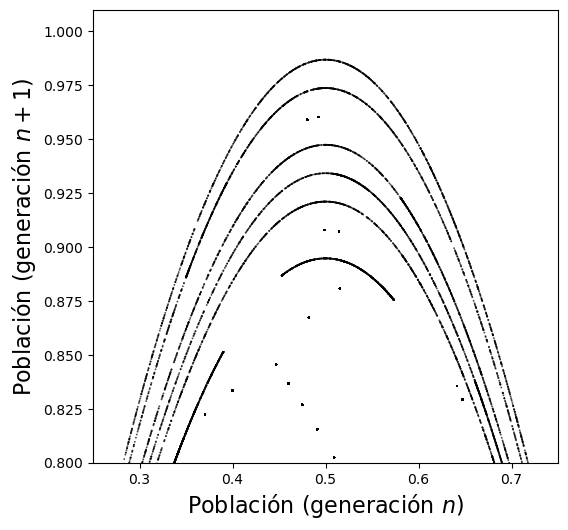
\includegraphics[width=0.5\columnwidth]{Ilustraciones/Cap_SFI/Diagramas fase.png}
    \caption{Diagrama fase que nos permite visualizar si el sistema se estabilida. Básicamente nos dice de dónde proviene y a dónde llega el estado del sistema.}
    \label{fig:diagrama_fase_logística}
\end{figure}

En la figura \ref{fig:diagrama_fase_logística}, cada arco representa la evolución de la ecuación logística \ref{eq:logísitca} a un valor de $\lambda$. Es interesante notar que los arcos nunca se cruzan. Cada uno tiene una evolución diferente a las demás.
Los pequeños arcos cerca del centro de la figura con sólo unos cuantos puntos (o incluso únicamente uno) representan los casos donde el sistema converge rápidamente a un punto o un ciclo límite.

\subsubsection{Sistemas de Funciones iteradas y mapeo de Henón}

Los sistemas de funciones iteradas son un tipo particular de ecuaciones diferenciales discretas en cuanto a que su estructura básica es la misma que en \ref{eq:iteraciones}. Usualmente se les asocia con conjuntos autosemejantes aunque hay ciertas condiciones que deben cumplirse para que esto ocurra. 
\\

Unos de los sitemas de funciones iteradas más estudiados es el mapeo de Henón cuyas coordenadas a cada iteraciones se obtienen mediante las ecuaciones:

\begin{equation}
    \begin{cases}
    x_{n+1} = 1 - a \, x_{n}^{2} + y_{n} \\
    y_{n+1} = b \, x_{n}
    \end{cases}
    \label{eq:henon}
\end{equation}



\subsubsection{Juego del caos}

El juego del caos, similar a los sistemas dinámicos discretos, consiste en un conjunto de condiciones iniciales y una función o acción a repertirse.

Uno de los más emblemáticos es el \textit{Triángulo de Sierpinski} donde, sobre un triángulo equilátero con vértices $V = \{ v_{1} = (x_{1}, y_{1}), v_{2} = (x_{2}, y_{2}), v_{3} = (x_{3}, y_{3}) \}$ y etiquetados por $V_{e}$ = \( \{1,2,3\} \), se aplica el siguiente algoritmo:

\begin{enumerate}
    \item Se elige aleatoriamente un número $\kappa \in V_{e}$ y se genera con ello el punto inicial ($p_{0} = v_{\kappa}$) que esté entre los vértices de $V$.
    \item Se elige aleatoriamente una nueva etiqueta $\kappa_{1} \in V_{e}$ y se calcula el punto medio entre $p_{0}$ y $v_{\kappa_{1}}$. Este nuevo punto es $p_{1}$, el correspondiente a la iteración $1$. Más suscintamente, $p_{1} = PM(p_{0}, v_{\kappa_{1}})$.
    \item Se itera el paso anterior con una sutil pero importante diferencia: no se toma nuevamente $p_{0}$ para calcular el punto medio sino el punto generado durante la previa iteración. Es decir, $p_{n+1} = PM(p_{n}, v_{\kappa_{n+1}})$ para $n \geq 1$.
\end{enumerate}

Se muestra en la figura \ref{fig:Sier_sub1} la gráfica de los puntos resultantes de cinco iteraciones; se puede inferir cuál fue la secuencia de etiquetas que los generó: $\{ 1,3,1,2,3,2 \}$. La gráfica en \ref{fig:Sier_sub2} se obtuvo con un millón de iteraciones y se puede decir que ningún punto cayó dentro del triángulo blanco invertido que está en el centro de la figura y que es semejante al original. Más aún, en \ref{fig:Sier_sub3} se cambiaron los colores de tres triángulos más pequeños para evidenciar que éstos, a su vez, tienen triángulos blancos invertidos todos ellos semejantes. 


\begin{figure}[h]
\centering
\begin{subfigure}{.3\textwidth}
  \centering
  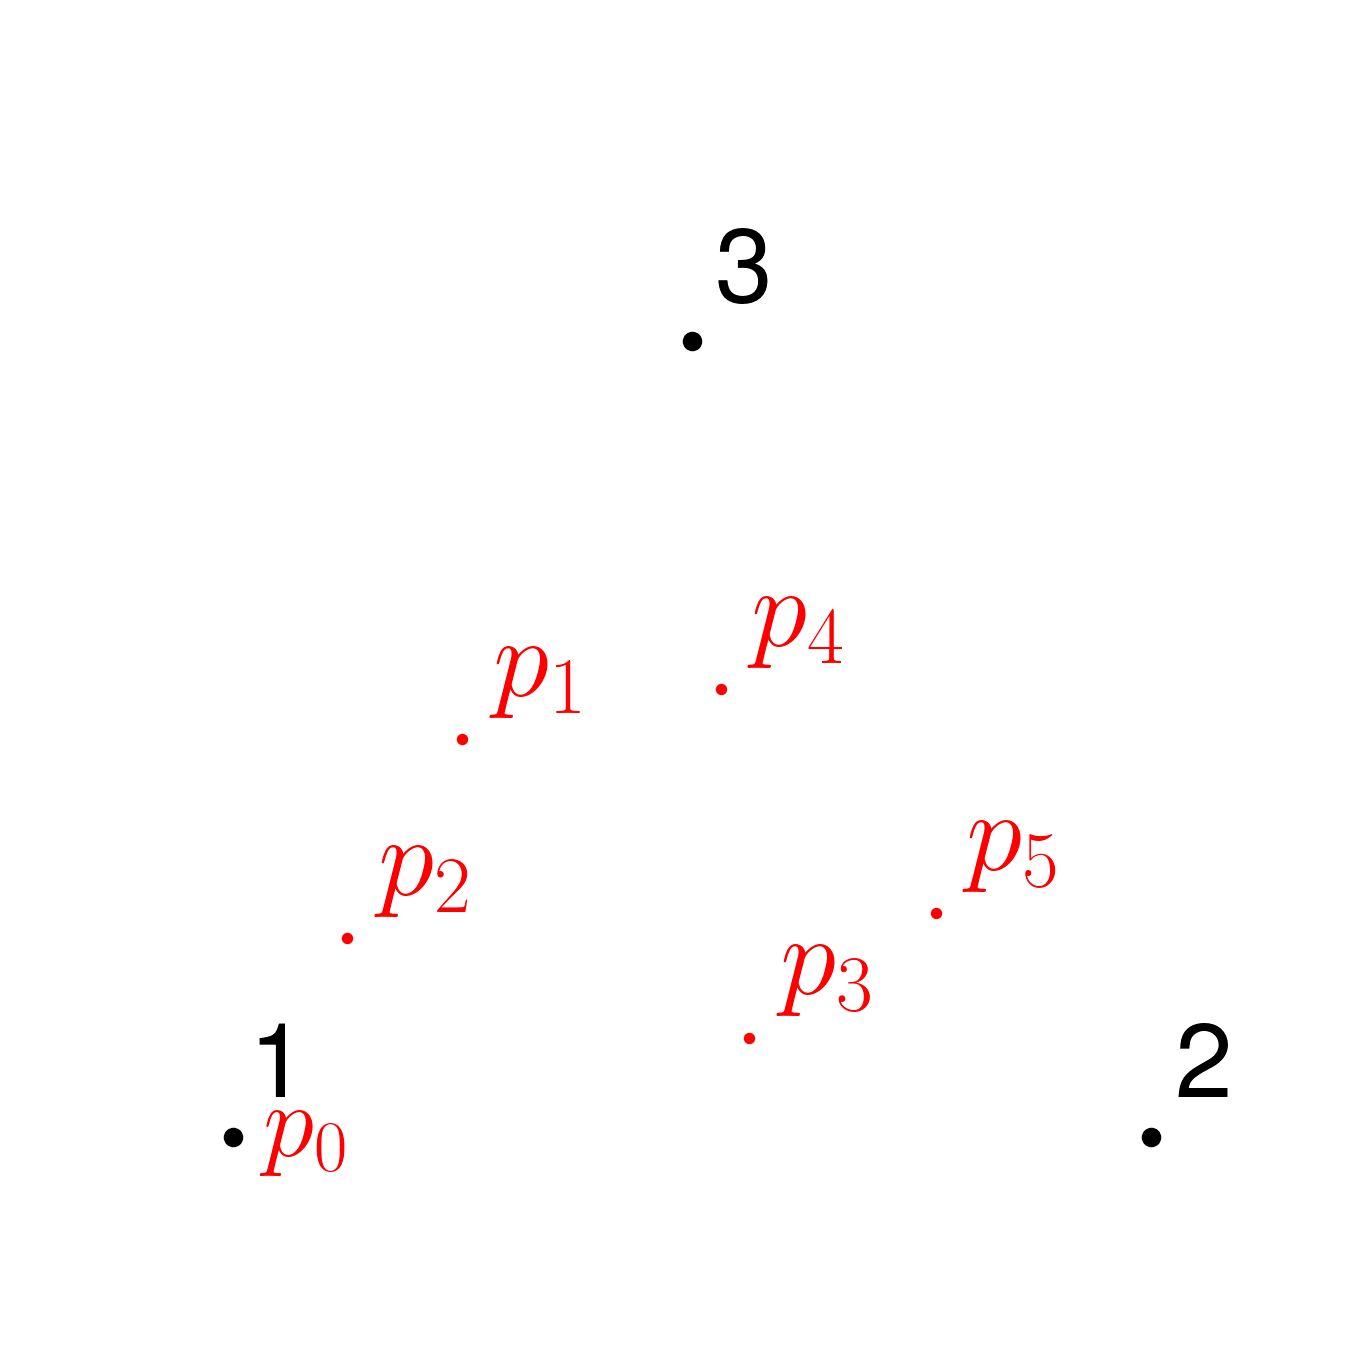
\includegraphics[width=1\linewidth]{Ilustraciones/Cap_SFI/Sierpinski_Iteraciones.png}
  \caption{}
  \label{fig:Sier_sub1}
\end{subfigure}%
\begin{subfigure}{.3\textwidth}
  \centering
  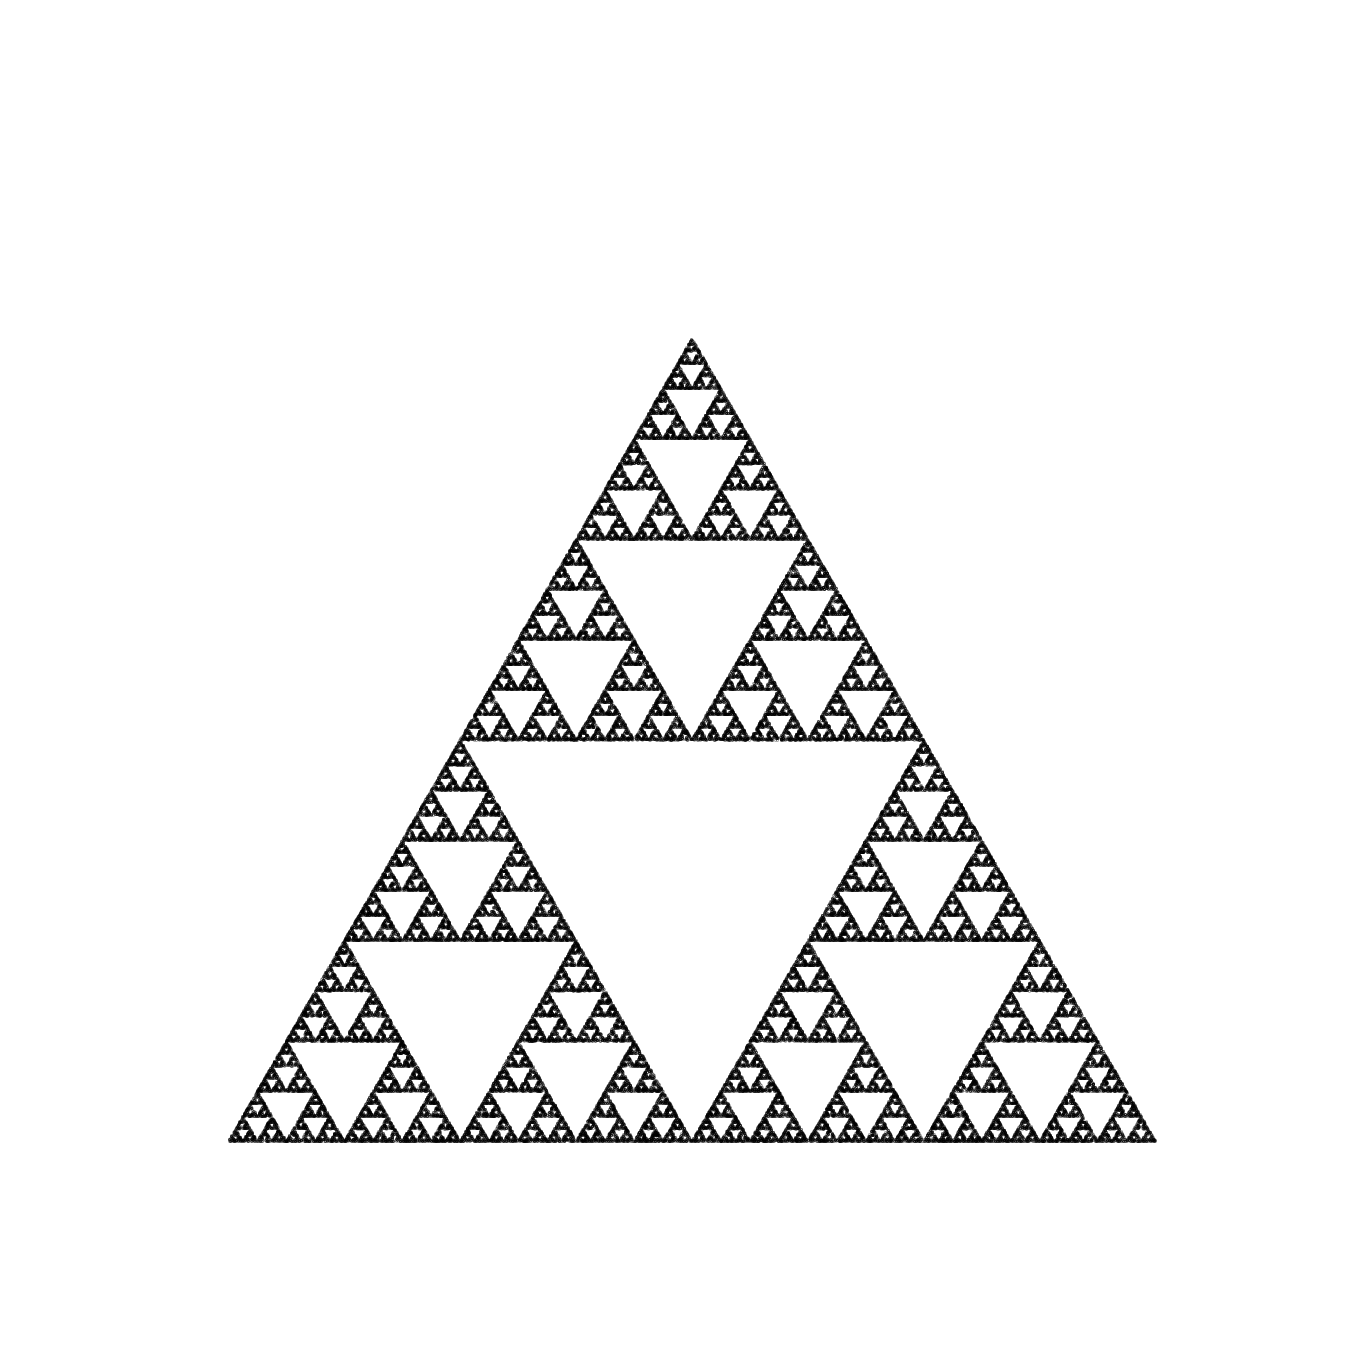
\includegraphics[width=1\linewidth]{Ilustraciones/Cap_SFI/Sierpinski_Final.png}
  \caption{}
  \label{fig:Sier_sub2}
\end{subfigure}%
\begin{subfigure}{.3\textwidth}
  \centering
  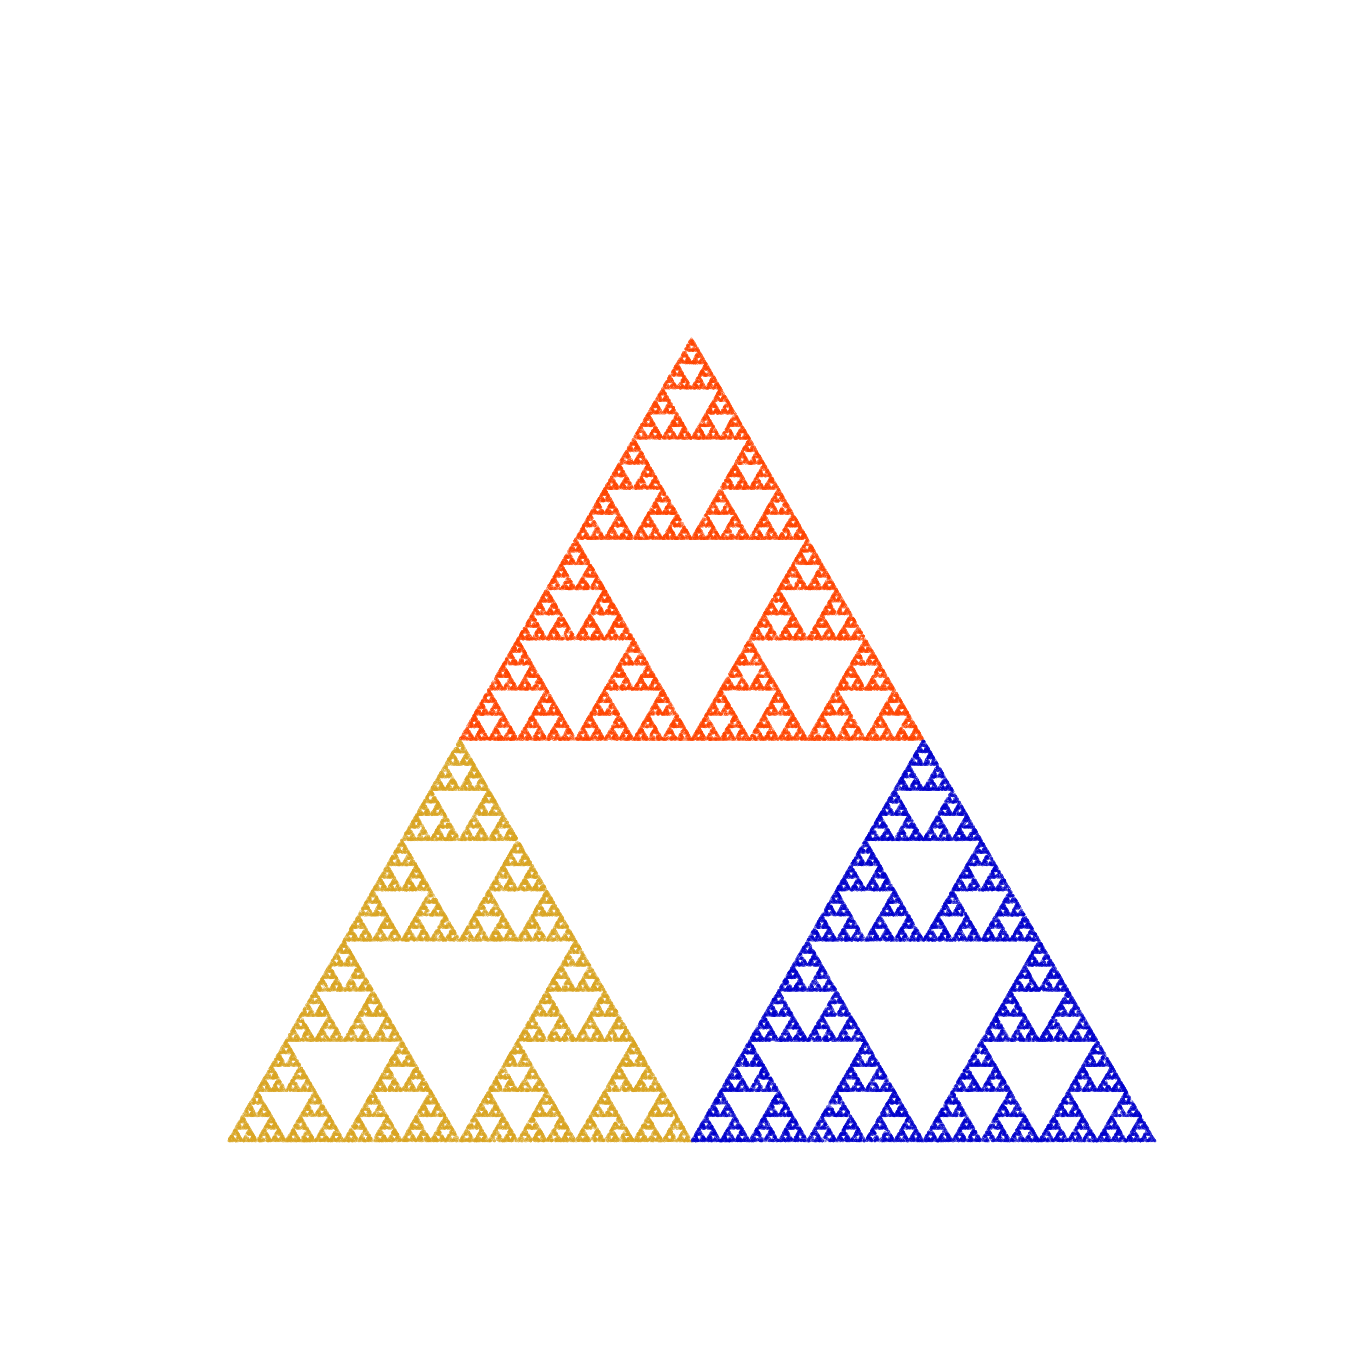
\includegraphics[width=1\linewidth]{Ilustraciones/Cap_SFI/Sierpinski_Fractal_Highlight.png}
  \caption{}
  \label{fig:Sier_sub3}
\end{subfigure}
\caption{(a): Cinco puntos generados con el algoritmo del triángulo de Sierpinski. (b): Gráfica de los puntos después de un millón iteraciones. (c): Los tres triángulos pequeños reproducen la forma del original en (b), la gráfica es auto-semejante.}
\label{fig:Sierpinski}
\end{figure}


\subsection*{Juego del Caos en el DNA}

El DNA yace dentro de cada célula de cada ser vivo. Tiene la información suficiente para que la célula cumpla con las todas funciones necesarias para sustentar la vida. Es una macromolécula que forma una espiral y en cuyo interior hay únicamente cuatro posibles moléculas, llamadas nucleótidos: Adenina, Guanina, Citosina, Timina. De ahora en adelante abreviaremos estos elementos con el diccionario: \{Adenina: A, Guanina: G, Citosina: C, Timina: T\}.

Para fines prácticos, consideraremos que el DNA es únicamente una larga cadena de caracteres donde a cada posición la ocupa alguno de los elementos del diccionario de arriba.
\\

El juego del caos en el DNA consiste en:

\begin{itemize}
\item A cada vértice de un cuadrado se le etiqueta con uno de los elementos del diccionario ${A, T, C, G}$ de modo que a cada vértice le corresponda únicamente un elemento del diccionario.
\item Se identifica la letra que ocupa la primera posición dentro de la secuencia y se coloca un punto sobre el vértice que la representa en el cuadrado del paso anterior. A este punto inicial lo llamamos $x_{0}$.
\item Se identifica la letra que le sucede a la del punto anterior y se coloca un nuevo punto ($x_{1}$) en el punto medio entre $x_{0}$ y el vértice que representa dicha letra. 
\item Se itera la acción anterior. Se fija qué letra ocupa la posición $n$ de la cadena y se traza el punto medio entre el punto $x_{n-1}$ y el vértice que representa a la letra en la posición $n$.
\end{itemize}
\\

Tomemos, a modo de ejemplo, la siguiente sub-cadena del DNA:

\begin{center}
\textbf{ATGCCGATA}
\end{center}

En la figura \ref{fig:DNA_chaos_game} se ilustra cómo luce la gráfica del algoritmo para las primera 9 posiciones de la cadena.

%También se muestra en la figura \ref{fig:config} las seis diferentes maneras de etiquetar los vértices de un cuadrado con los cuatro elementos del diccionario sin que alguna sea una reflección simple de cualquier otra.
\\

%Esto último se incluye porque, si bien la elección de las etiquetas es arbitraria, se consideran los seis posibles casos para identificar patrones o similitudes entre ellas.


\begin{figure}[h!]
    \centering
    \includegraphics[width=0.75\columnwidth]{Ilustraciones/Cap_SFI/Caos_biología_flechas.png}
    \caption{Algoritmo del juego del caos en secuencias de genomas. Se muestran los primeros nueve puntos del}
    \label{fig:DNA_chaos_game}
\end{figure}


%\begin{figure}[h!]

%\begin{minipage}{.3\linewidth}
%\centering
%\subfloat[]{\label{main:a}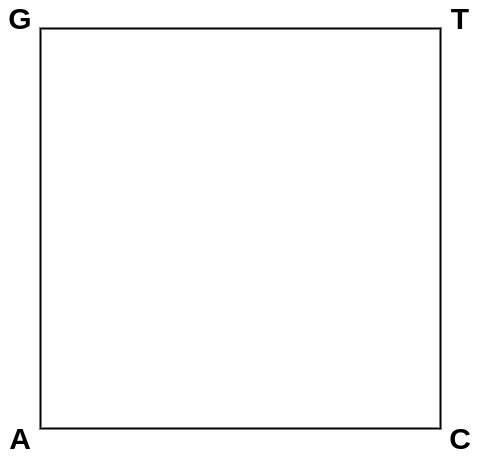
\includegraphics[scale=.25]{Ilustraciones/Cap_SFI/dic01.png}}
%\end{minipage}%
%\begin{minipage}{.3\linewidth}
%\centering
%\subfloat[]{\label{main:a}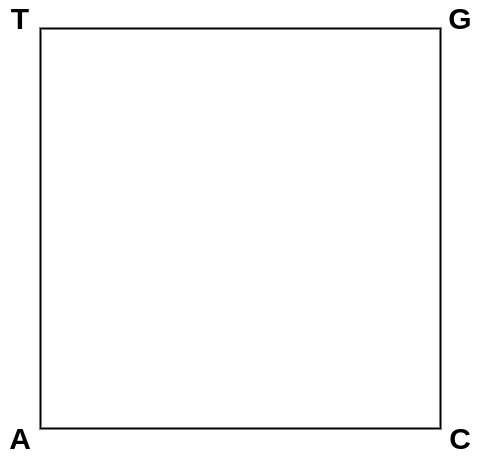
\includegraphics[scale=.25]{Ilustraciones/Cap_SFI/dic02.png}}
%\end{minipage}%
%\begin{minipage}{.3\linewidth}
%\centering
%\subfloat[]{\label{main:b}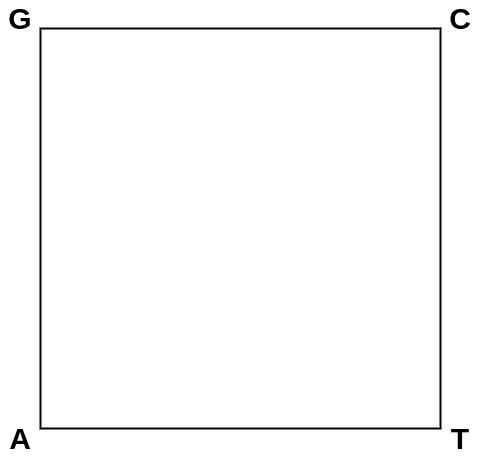
\includegraphics[scale=.25]{Ilustraciones/Cap_SFI/dic03.png}}
%\end{minipage}\par\medskip


%\begin{minipage}{.3\linewidth}
%\centering
%\subfloat[]{\label{main:a}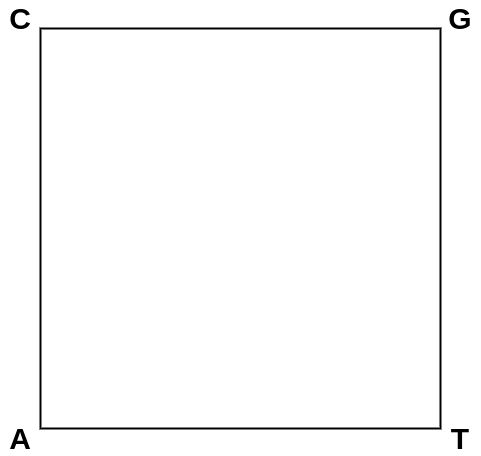
\includegraphics[scale=.25]{Ilustraciones/Cap_SFI/dic04.png}}
%\end{minipage}%
%\begin{minipage}{.3\linewidth}
%\centering
%\subfloat[]{\label{main:a}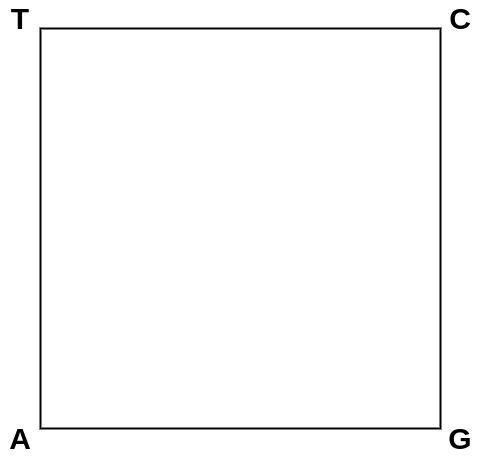
\includegraphics[scale=.25]{Ilustraciones/Cap_SFI/dic05.png}}
%\end{minipage}%
%\begin{minipage}{.3\linewidth}
%\centering
%\subfloat[]{\label{main:b}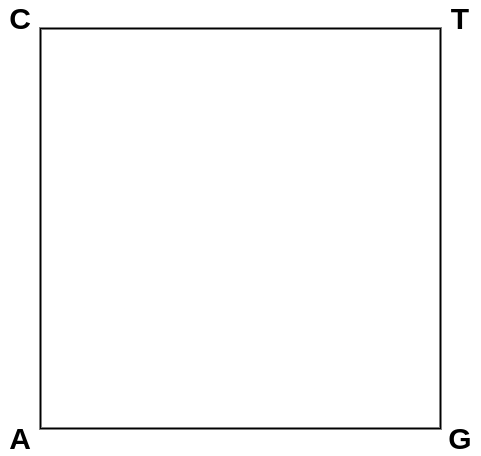
\includegraphics[scale=.25]{Ilustraciones/Cap_SFI/dic06.png}}
%\end{minipage}

%\caption{Seis configuraciones de vértices sobre los cuales se iteró el juego del caos con muestras de 1,000,000 puntos.}
%\label{fig:config}
%\end{figure}


\subsubsection{Fractales}

Los fractales son conjuntos cuya pricipal característica es que tienen una \textit{dimensión fraccionaria}. Otra manera de decir esto requiere que pensemos en las dimensiones como el número de veces que un objeto se replica a sí mismo cuando se aumenta o se reduce uno de sus lados como una potencia de $2$.
\\

La dimensión se calcula con la expresión: $2^{k} = M$ donde $k$ es la dimensión y $M$ es el número de copias resultantes de duplicar el tamaño de un objeto. Acomodando un poco la expresión anterior llegamos a que $k = \slashfracstyle{ln(M) / ln(2)}$.
\\

La figura \ref{fig:Dimensiones} ilustra cómo ésto se relaciona con la dimensión topológica. En \ref{fig:Dim_sub1}, duplicar el tamaño de un segmento de recta resulta en dos copias de la original, entonces $k = \slashfracstyle{ln(2) / ln(2)} = 1$. Cuando se lleva esta idea a un cuadrado como en  \ref{fig:Dim_sub2}, aumentar el tamaño del cuadrado en un factor de $2$ produce ahora cuatro copias de la figura inicial: $k = \slashfracstyle{ln(4) / ln(2)} = 2$. Finalmente en \ref{fig:Dim_sub3} se muestra únicamente la silueta de los tres triángulos de \ref{fig:Sier_sub3}. Duplicar las dimensiones del triángulo resulta en tres copias de éste, su dimensión es entonces $k = \slashfracstyle{ln(3) / ln(2)} \approx 1.584$. 


\begin{figure}[h]
\centering
\begin{subfigure}{.30\textwidth}
  \vspace{2cm}
  \centering
  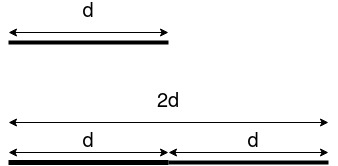
\includegraphics[width=1\linewidth]{Ilustraciones/Cap_SFI/Escalas_Linea.jpg}
  \caption{}
  \label{fig:Dim_sub1}
\end{subfigure}%
\begin{subfigure}{.30\textwidth}
  \centering
  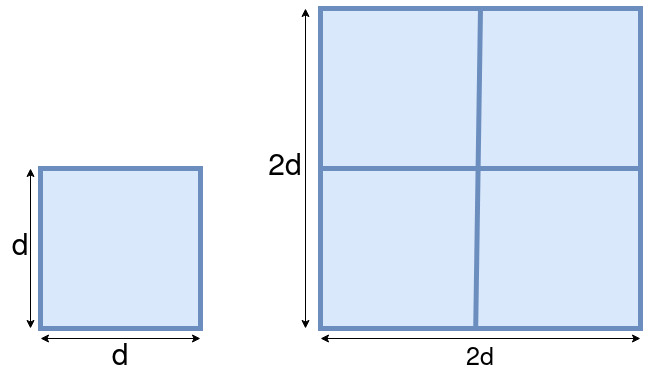
\includegraphics[width=1\linewidth]{Ilustraciones/Cap_SFI/Escala_cuadrado.jpg}
  \caption{}
  \label{fig:Dim_sub2}
\end{subfigure}%
\begin{subfigure}{.30\textwidth}
  \vspace{1.5cm}
  \centering
  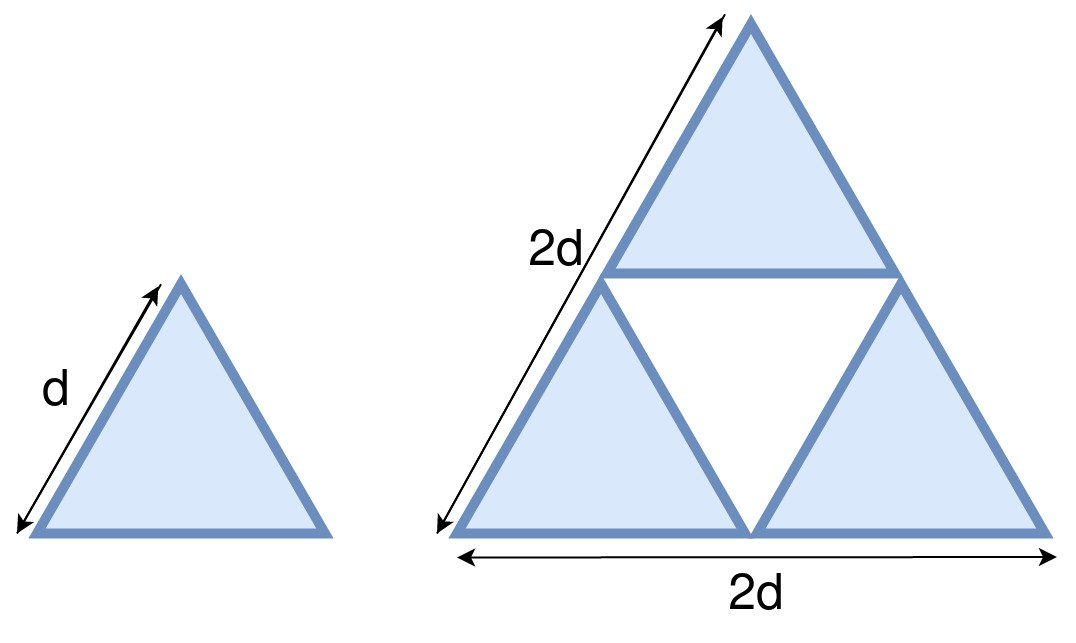
\includegraphics[width=1\linewidth]{Ilustraciones/Cap_SFI/Escala_cubo.jpg}
  \caption{}
  \label{fig:Dim_sub3}
\end{subfigure}
\caption{El cálculo de la dimensión fractal coincide con la topológica para una y dos dimensiones. El número de copias crece como potencia de $2$ al duplicar la longitud de un objeto. Cuando el conjunto es auto-semejante y no llena el espacio; la dimensión fractal no es un número entero.}
\label{fig:Dimensiones}
\end{figure}

Una de las implicaciones que esto tiene es que un fractal no necesariamente \textit{llena} el espacio donde se encuentra cuando se hacen copias de él, dejando espacios vacíos. La frontera del fractal suele describir vericuetos donde se puede verificar la autosemejanza, es decir, que el objeto se replica a sí mismo independientemente de la escala a la que se le observe.
\\

Resulta sencillo calcular la dimensión fractal de conjuntos con evidente autosemejanza aunque esta cualidad no siempre aparezca durante el estudio de sistemas dinámicos. En la siguiente sección se introduce la dimensión de Minkowski-Bouligand, un método numérico para el cálculo de la dimensión que aproxima la dimensión de fractales.

\subsubsection{Dimensión fractal y de Minkowski-Bouligand}

Si bien la manera de calcular la dimensión fractal con la definición y el conteo del número de réplicas que se genera de la figura al duplicar el tamaño de uno de los lados; tiene limitaciones cuando la autosemejanza es no trivial o incluso inexistente.
\\

Para calcular la dimensión fractal de conjuntos donde no sea posible contar el número de réplicas, se usa el algoritmo  de \textit{Minkowski-Bouligand} también conocido como el algoritmo de \textit{conteo de cajas}. También se basa en la expresión $2^{k} = M$ y busca particionar el espacio métrico dentro del cual se encuentra el conjunto en segmentos cuyo tamaño decrezca como pontencia de $\sim \frac{1}{2^{n}}$ y donde $n$ es un número natural sobre el cual se itera. 
\\


A medida que se particione el espacio métrico, se cuenta el número de cajas dentro de las cuales haya al menos un elemento del conjunto. La dimensión se calcula con la expresión:

\begin{equation}
    dim_{box}(\mathcal{S}) = \lim_{\epsilon \to \; 0} \frac{log (N(\epsilon))}{log(1/\epsilon)}
    \label{eq:dimfractal}
\end{equation}

Donde $\epsilon$ es la longitud de cada elemento de la partición y $N(\epsilon)$ es el número de cajas que contienen al menos un elemento del conjunto $R$.
\\

En la figura \ref{fig:box-count} se muestran las primeras cuatro iteraciones del algoritmo del conteo de cajas aplicado sobre el triángulo de Sierpinski. Se aprecia cómo después de unas cuantas iteraciones, hay cuadrados dentro del triángulo invertido del centro donde no hay elementos del conjunto.
\\

\begin{figure}[h!]

\begin{minipage}{.45\linewidth}
\centering
\subfloat[]{\label{main:a}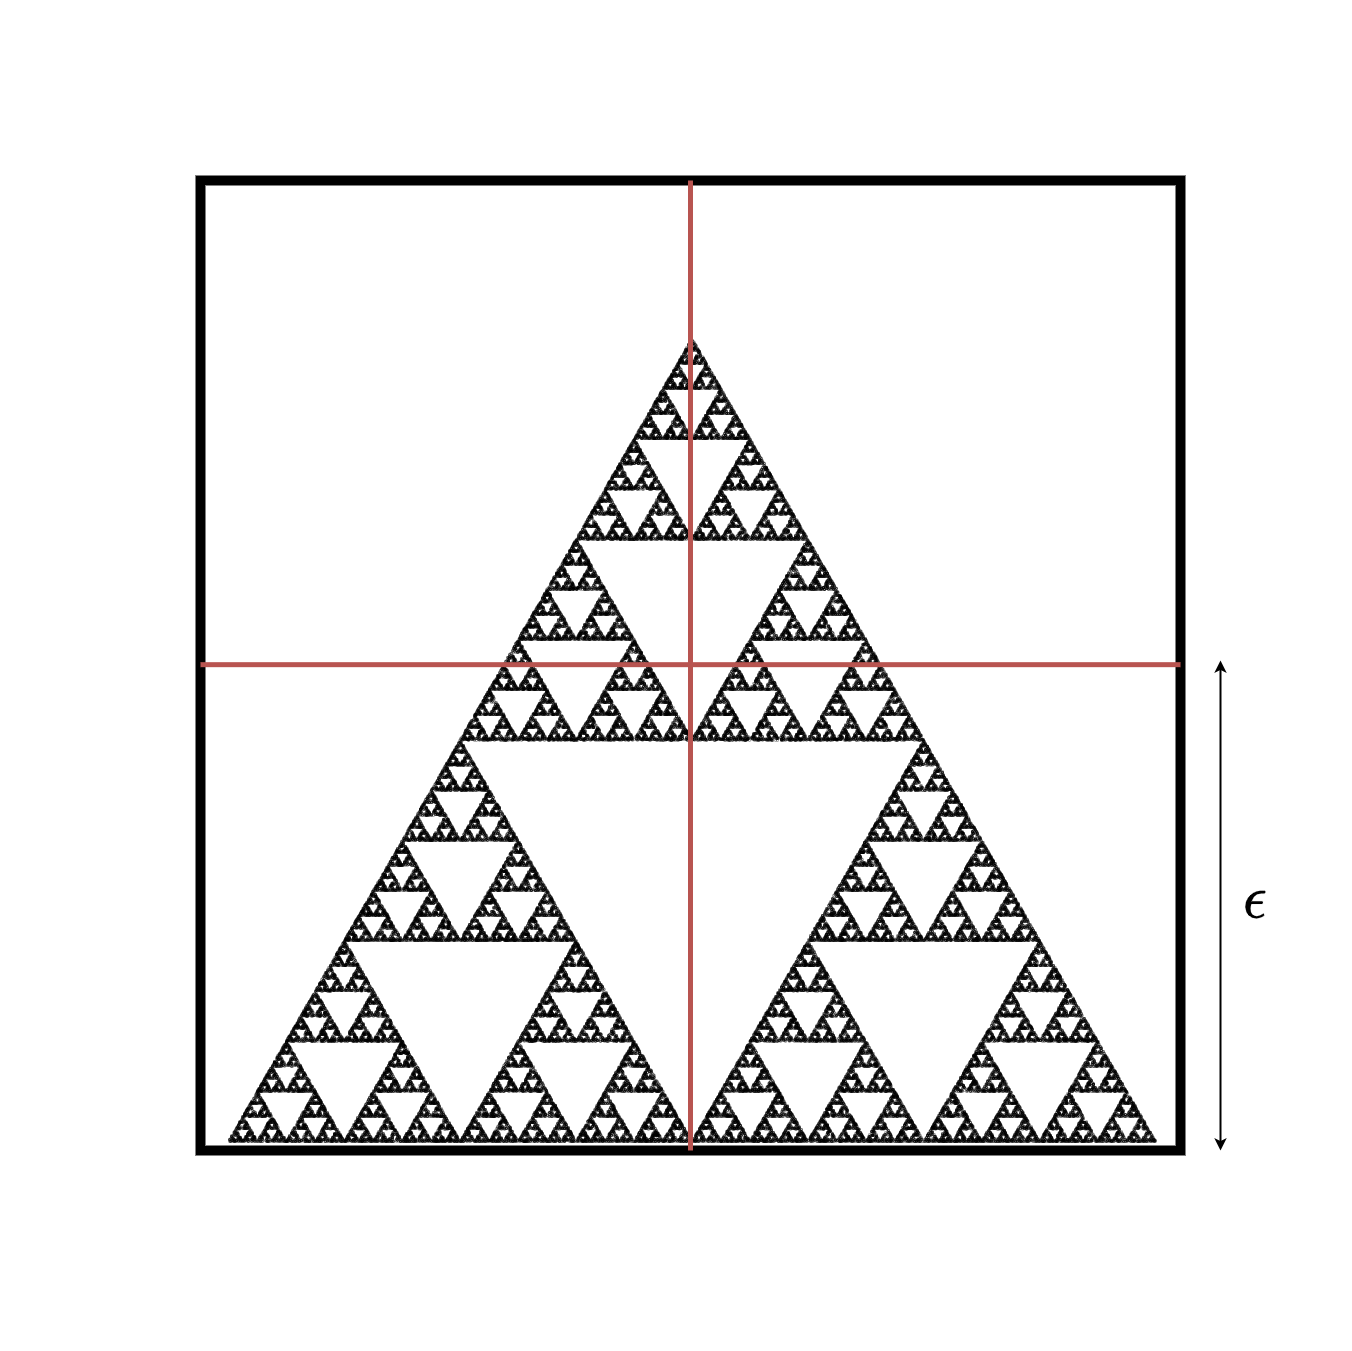
\includegraphics[scale=.15]{Ilustraciones/Cap_SFI/sier_fracdim01}}
\end{minipage}%
\begin{minipage}{.45\linewidth}
\centering
\subfloat[]{\label{main:b}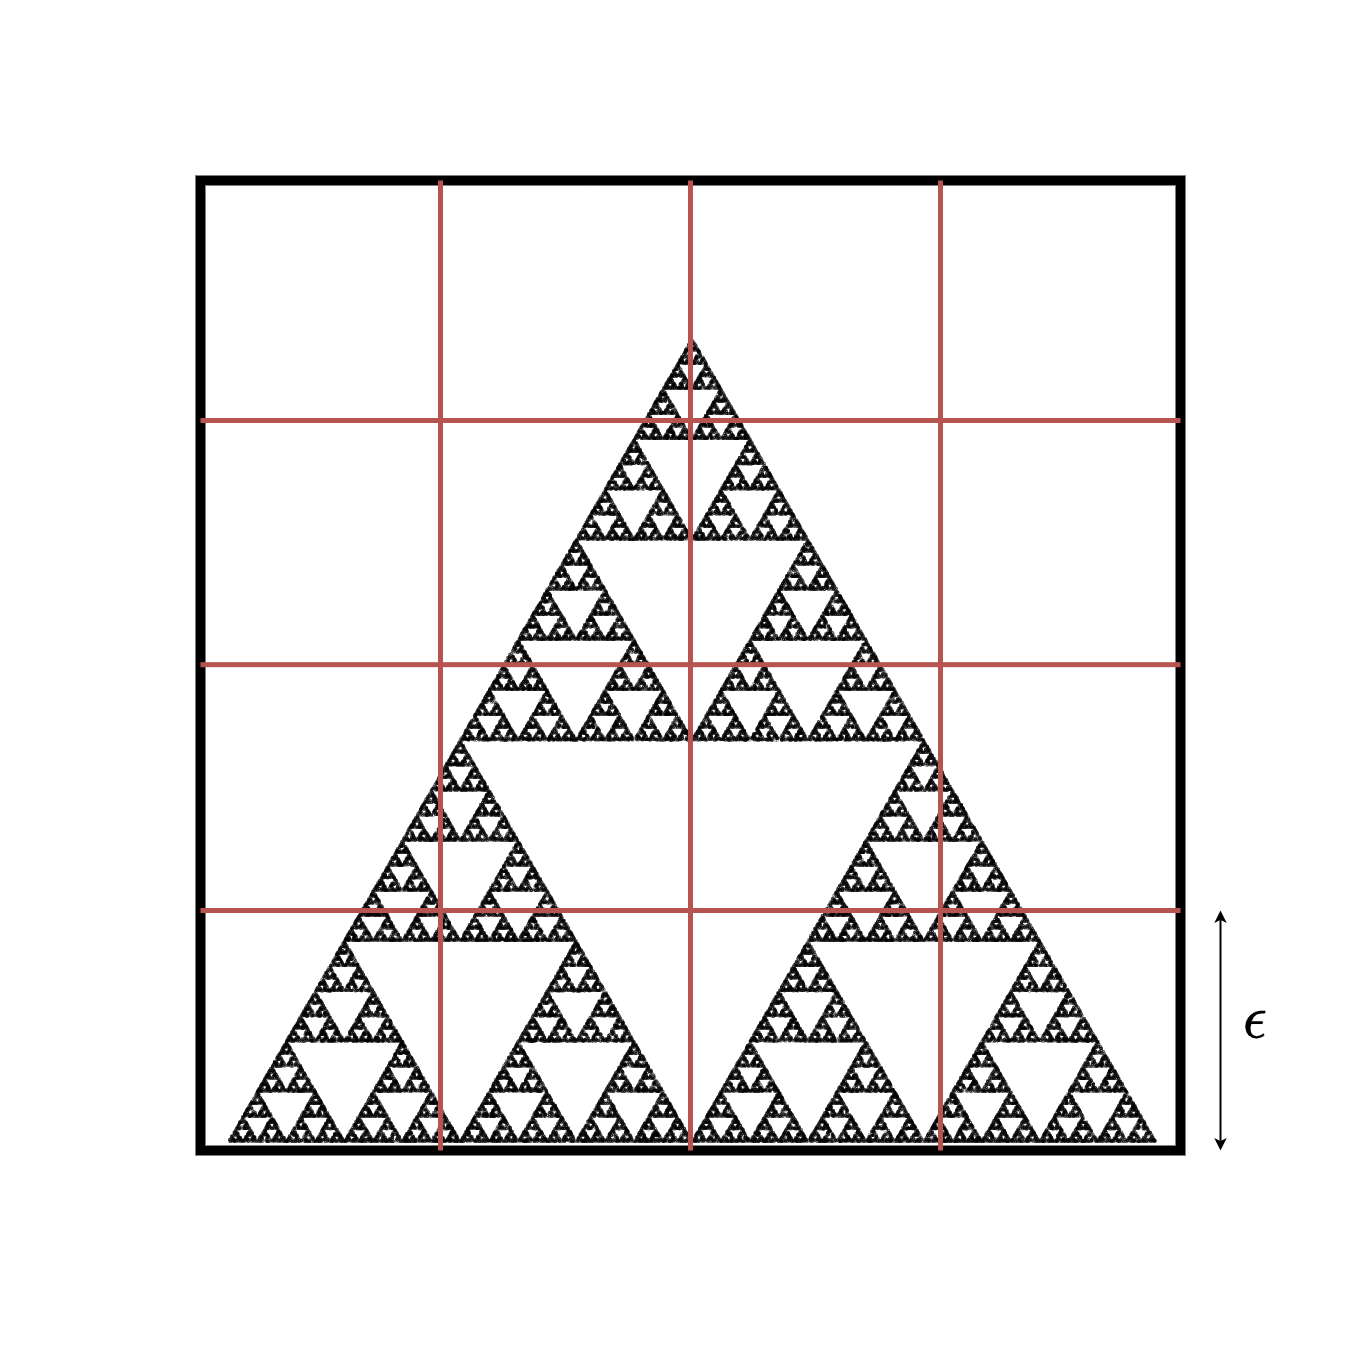
\includegraphics[scale=.15]{Ilustraciones/Cap_SFI/sier_fracdim02}}
\end{minipage}\par\medskip


\begin{minipage}{.45\linewidth}
\centering
\subfloat[]{\label{main:a}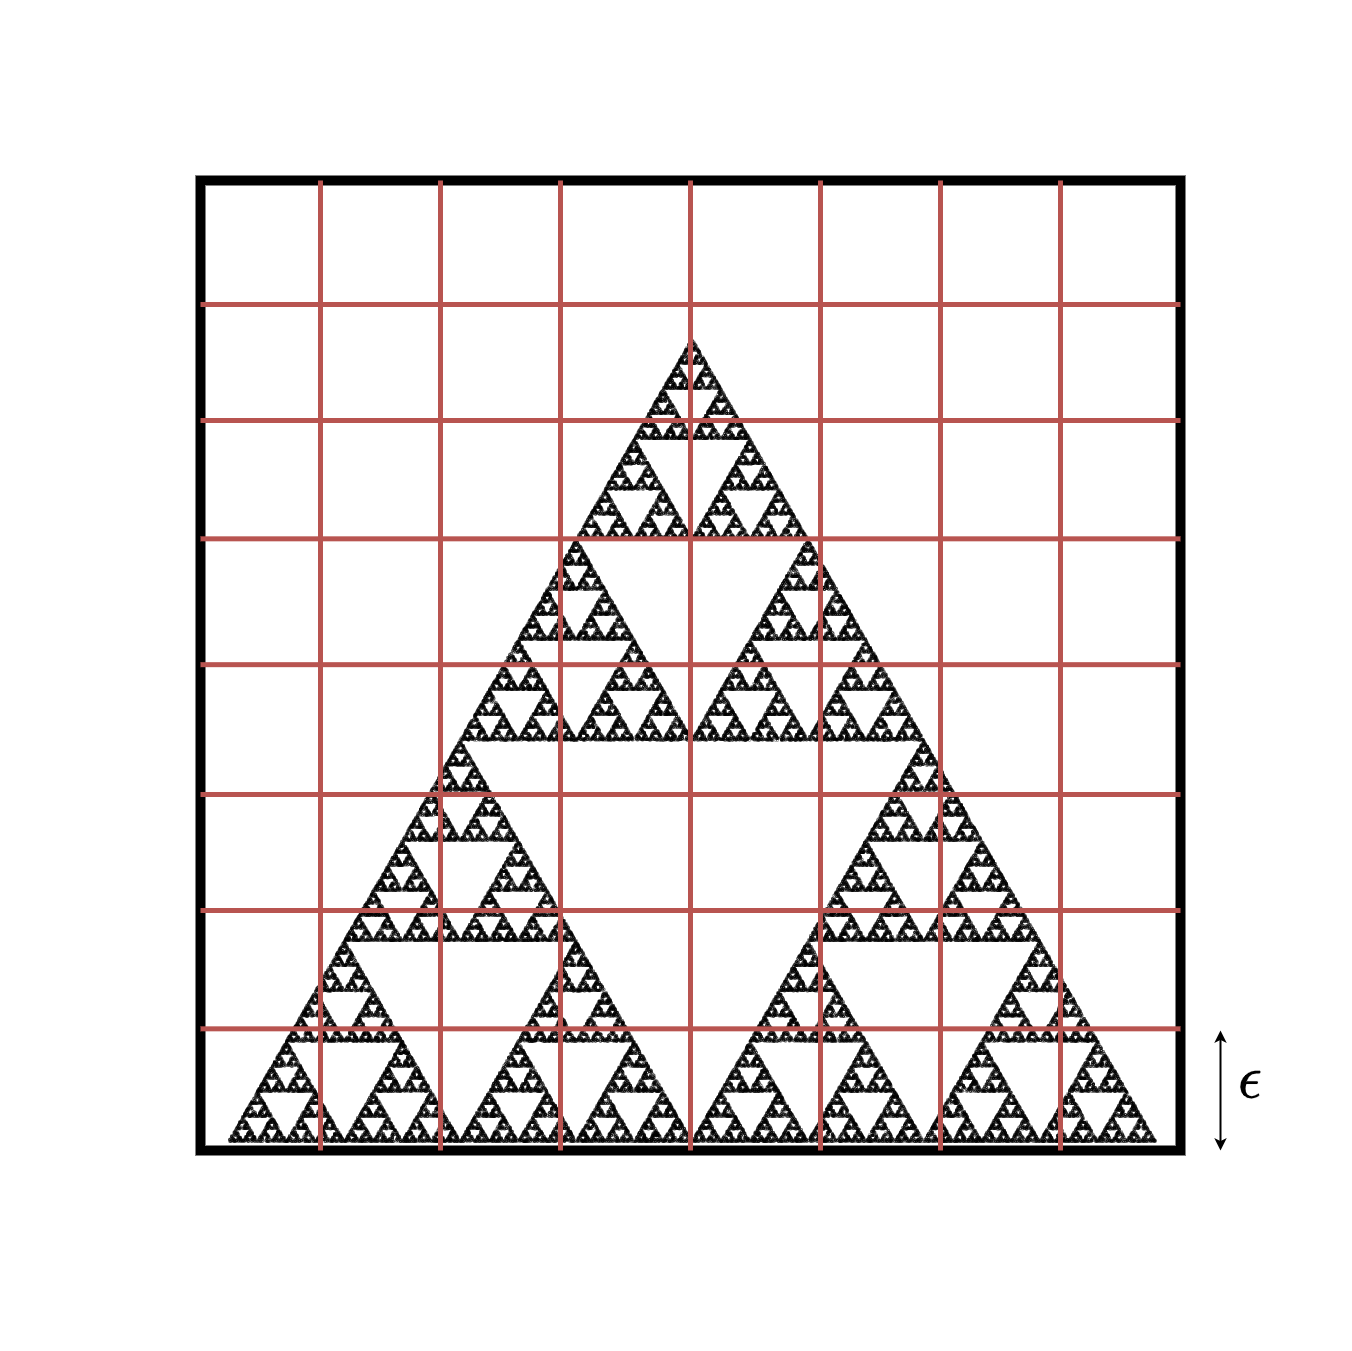
\includegraphics[scale=.15]{Ilustraciones/Cap_SFI/sier_fracdim03}}
\end{minipage}%
\begin{minipage}{.45\linewidth}
\centering
\subfloat[]{\label{main:b}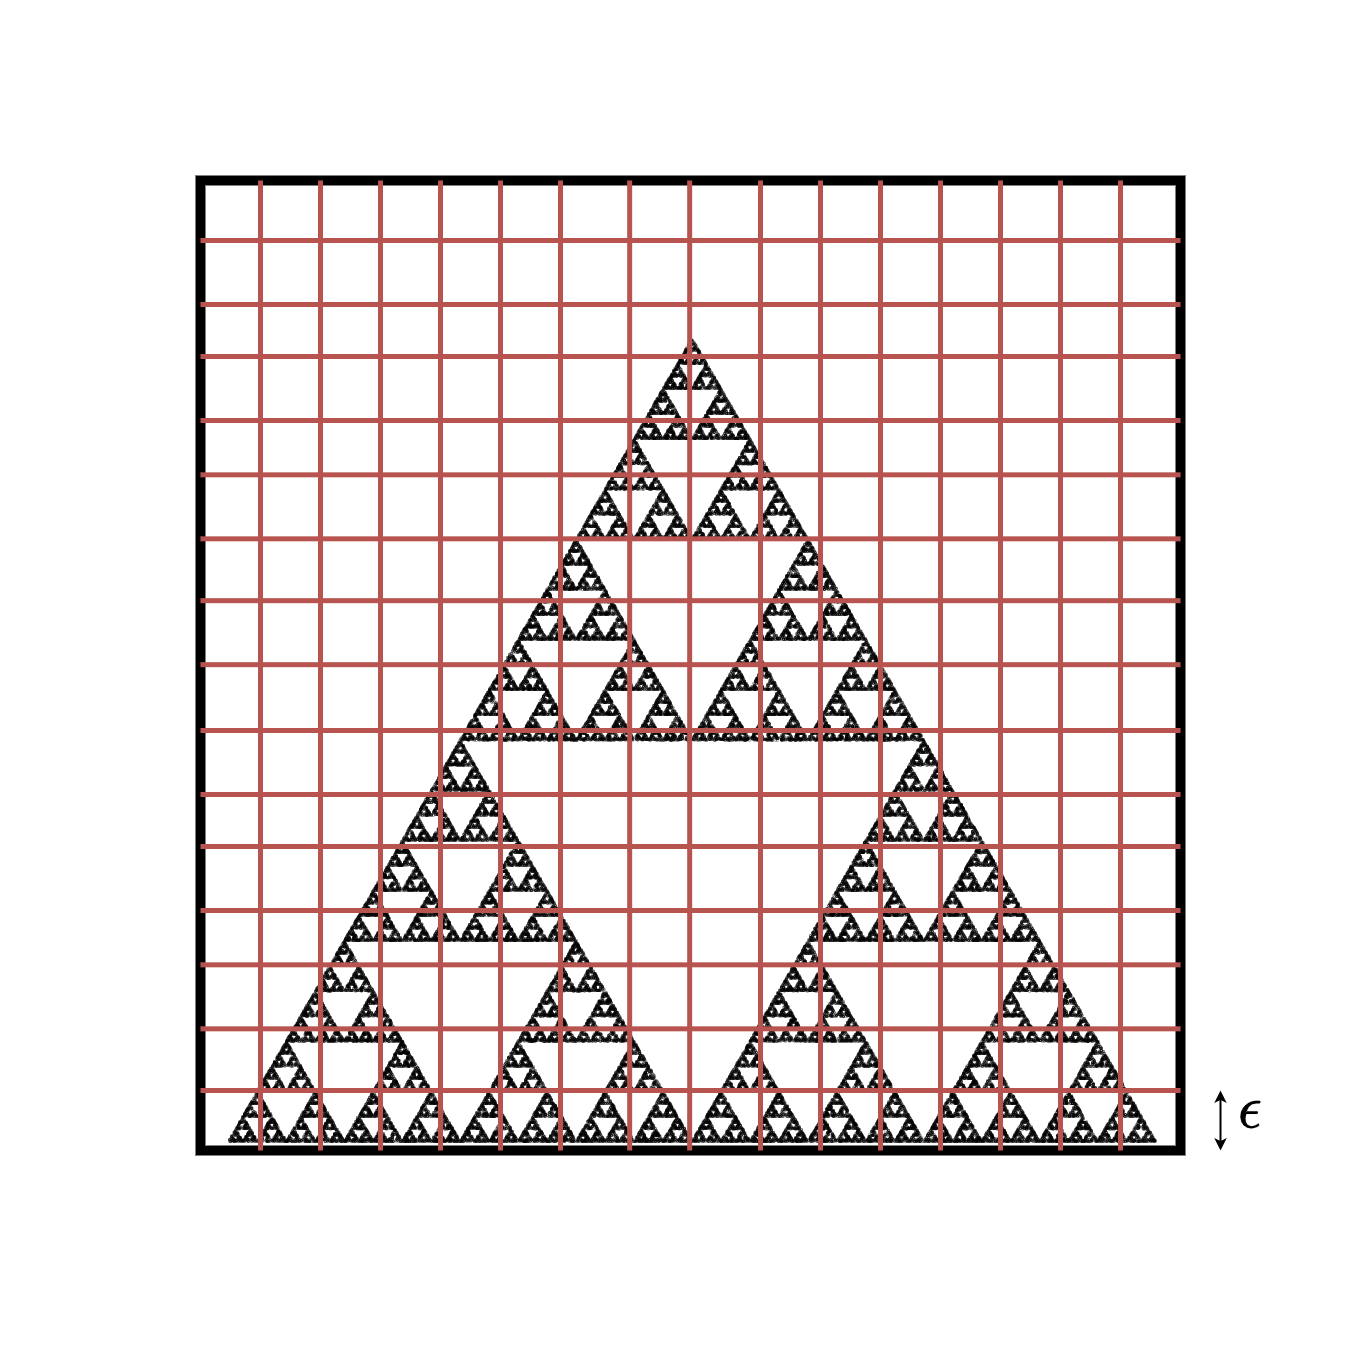
\includegraphics[scale=.15]{Ilustraciones/Cap_SFI/sier_fracdim04}}
\end{minipage}

\caption{Particiones del espacio que contiene al conjunto. El número de particiones dentro de $\mathbf{R^{2}}$ incrementa como función de $2^{n}$. A cada iteración se cuenta el número de \textit{cuadrados} que tengan al menos un elemento del conjunto $\mathcal{S}$ en su interior.}
\label{fig:box-count}
\end{figure}
\\

La manera de implementar la ecuación \ref{eq:dimfractal} para el cálculo de la dimensión consiste en iterar para diferentes valores escalas de $\epsilon$ y registrar $N(\epsilon)$. Luego se traza una recta con los valores de $log(1/\epsilon)$ sobre el eje de las $x$ y $log (N(\epsilon))$ sobre el eje de las $y$.
\\

Esto resulta en una recta cuya pendiente aproximará la dimensión fractal que deseamos calcular. De modo que se hace una regresión lineal con los puntos que resulten de la iteración para diferentes escalas de $\epsilon$.



\chapter{Implementación}

Se desarrolló un proyecto en el lenguaje de programación python 3.x que calcula la dimensión de Minkowski-Bouligand de cualquier subonjunto de $\mathrm{R^{2}}$ dadas sus coordinadas. Se probó el algoritmo con los siguientes conjuntos:

\begin{itemize}
    \item Una recta.
    \item Un cuadrado.
    \item Triángulo de Sierpinski.
    \item Conjunto de Henón
    \item Código de barras.
    \item Juego del caos en una subcadena del cromosoma 19.
    \item Juego del caos en una cadena aleatoria con el mismo diccionario del DNA.
\end{itemize}

Puede modificarse el número de elementos y extenderse para cualquier la dimensión de cualquier otro conjunto mediante la ejecución del método Frac_dimension_computation() incluído en la documentación del proyecto, mismo que puede encontrarse \href{https://github.com/RobertoBastida/ChaosGame_DNA}{\emph{dando click aquí}}.
\\

Se usó este desarrollo para reproducir el juego del caos en subcadenas del cromosoma 19 de longitud variable. También se generaron cadenas aleatorias a partir del diccionario de nucleótidos y se reprodujo el juego del caos en éstas también.

A cada uno de los conjuntos antes mencionados se le calculó la dimensión de Minkowski-Bouligand con el fin de indagar en la convergencia de la dimensión entre conjuntos aleatorios y conjuntos con cierto arreglo a partir del DNA real.
\\

Las longitudes de la subcadena del cromosoma 19 que se usaron para el experimento fueron: [$10^{4}$, $10^{5}$, $10^{6}$, $10^{7}$, $10^{8}$] y las longitudes de la cadena generada aleatoriamente fueron: [$10^{4}$, $10^{5}$, $10^{6}$, $10^{7}$]. Esto se hizo así porque se observó que la convergencia en la dimensión para el caso de la cadena aleatoria siempre ocurría entre las potencias $10^{5}$ y $10^{6}$. Además que el equipo de cómputo donde se desarrolló el proyecto tenía dificultades al generar la cadena de caracteres de longitud $10^{8}$.
\\


%%%%%%%%%%%%%%%%%%%%%%%%%%%%%%%%%%
%%%%%%%%%%%%%%%%%%%%%%%%%%%%%%%%%%
%%%%%%%%%%%%  19  %%%%%%%%%%%%
%%%%%%%%%%%%%%%%%%%%%%%%%%%%%%%%%%
%%%%%%%%%%%%%%%%%%%%%%%%%%%%%%%%%%

\begin{figure}[h!]

\begin{minipage}{.3\linewidth}
\centering
\subfloat[]{\label{main:a}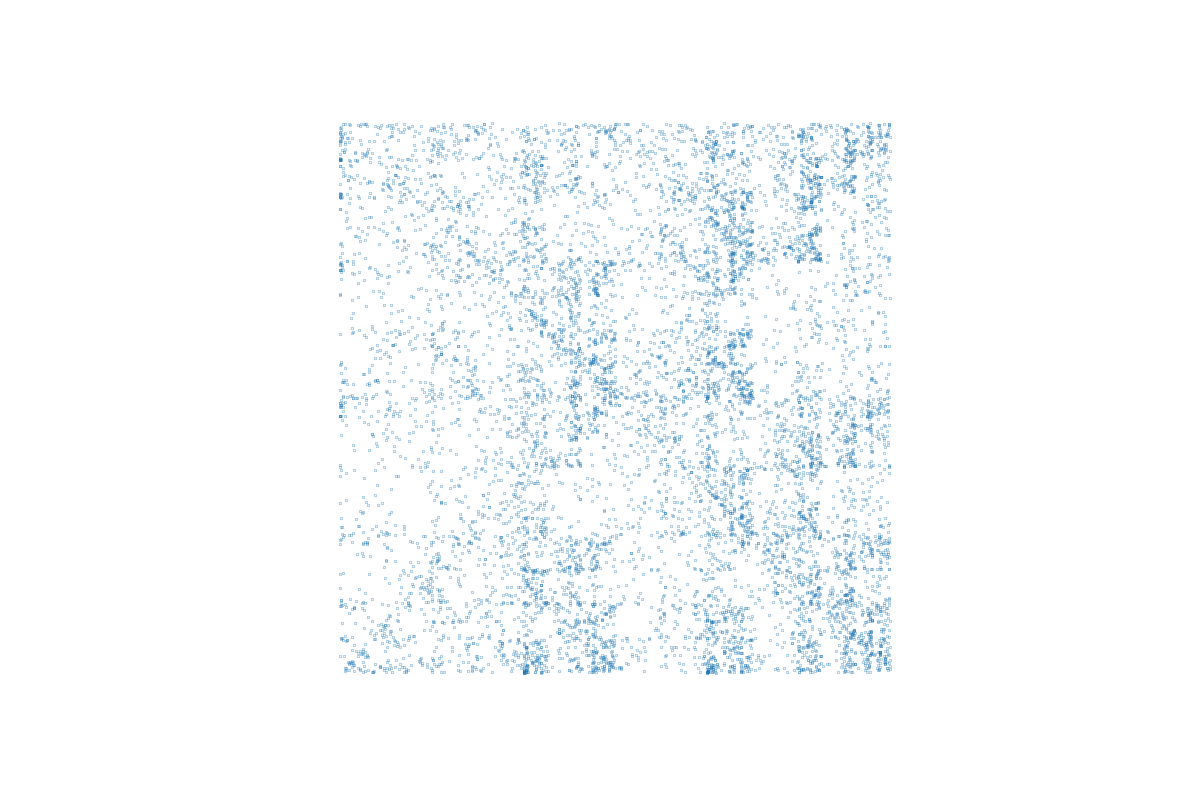
\includegraphics[scale=.45]{Ilustraciones/Cap_SFI/chr_19_0}}
\end{minipage}%
\begin{minipage}{.3\linewidth}
\centering
\subfloat[]{\label{main:a}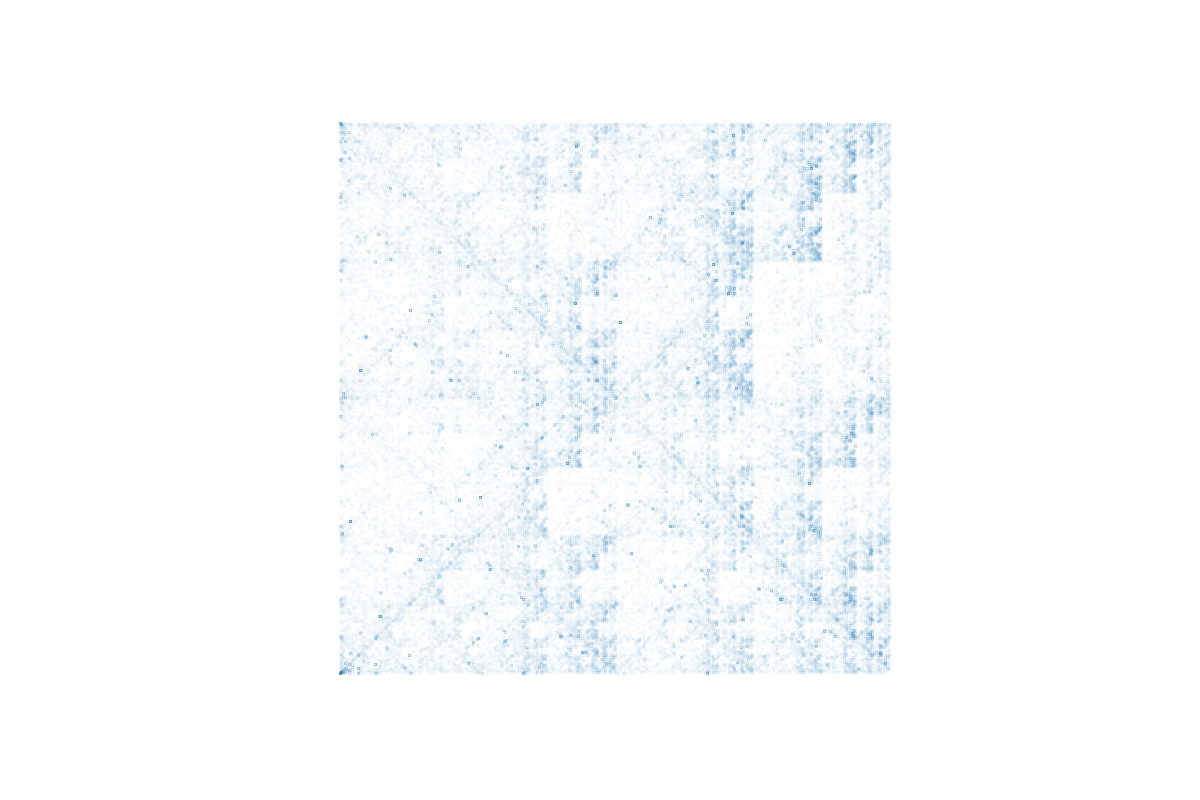
\includegraphics[scale=.45]{Ilustraciones/Cap_SFI/chr_19_1}}
\end{minipage}%
\begin{minipage}{.3\linewidth}
\centering
\subfloat[]{\label{main:b}
\includegraphics[scale=.45]{Ilustraciones/Cap_SFI/chr_19_2}}
\end{minipage}\par\medskip

\centering
\begin{minipage}{0.3\linewidth}
\centering
\subfloat[]{\label{main:a}
\includegraphics[scale=.45]{Ilustraciones/Cap_SFI/chr_19_3}}
\end{minipage}%
\begin{minipage}{0.3\linewidth}
\centering
\subfloat[]{\label{main:a}
\includegraphics[scale=.45]{Ilustraciones/Cap_SFI/chr_19_4}}
\end{minipage}

\caption{Gráficas del juego del caos aplicado a sub-cadenas del cromosoma 19. }
\label{fig:CG_chr19}
\end{figure}


\begin{figure}[h!]

\begin{minipage}{.3\linewidth}
\centering
\subfloat[]{\label{main:a}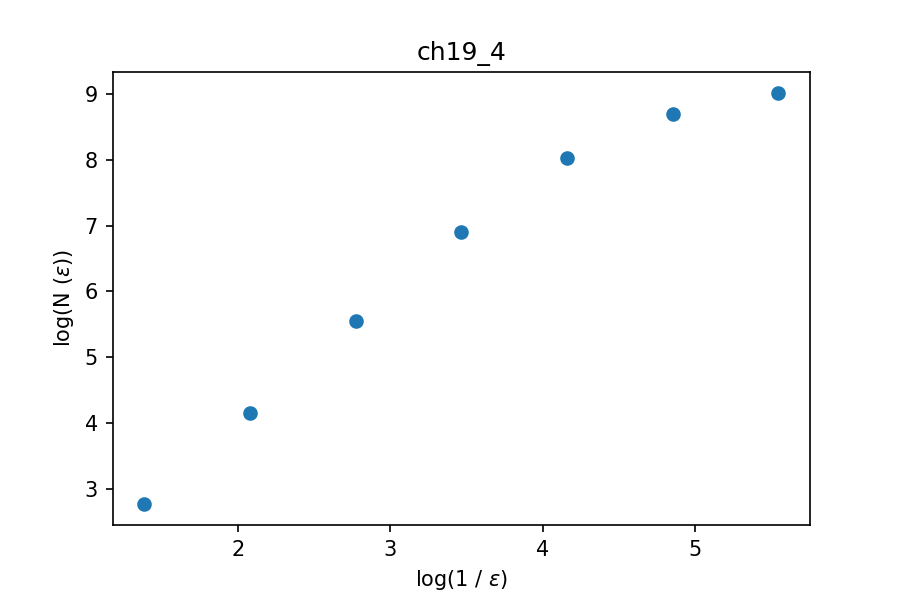
\includegraphics[scale=.35]{Ilustraciones/Cap_SFI_duplicates/chr_19_0.png}}
\end{minipage}%
\begin{minipage}{.3\linewidth}
\centering
\subfloat[]{\label{main:a}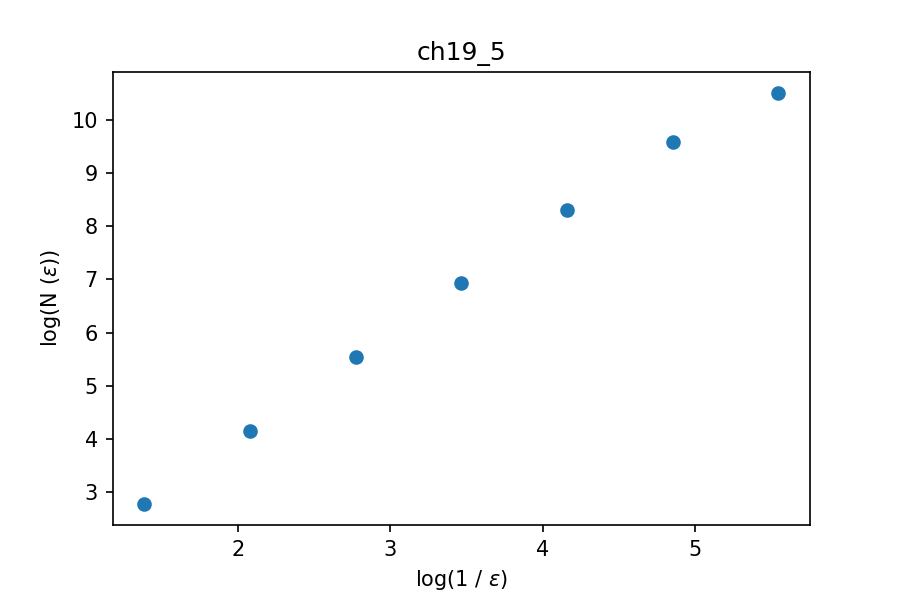
\includegraphics[scale=.35]{Ilustraciones/Cap_SFI_duplicates/chr_19_1.png}}
\end{minipage}%
\begin{minipage}{.3\linewidth}
\centering
\subfloat[]{\label{main:b}
\includegraphics[scale=.35]{Ilustraciones/Cap_SFI_duplicates/chr_19_2.png}}
\end{minipage}\par\medskip

\centering
\begin{minipage}{0.3\linewidth}
\centering
\subfloat[]{\label{main:a}
\includegraphics[scale=.35]{Ilustraciones/Cap_SFI_duplicates/chr_19_3.png}}
\end{minipage}%
\begin{minipage}{0.3\linewidth}
\centering
\subfloat[]{\label{main:a}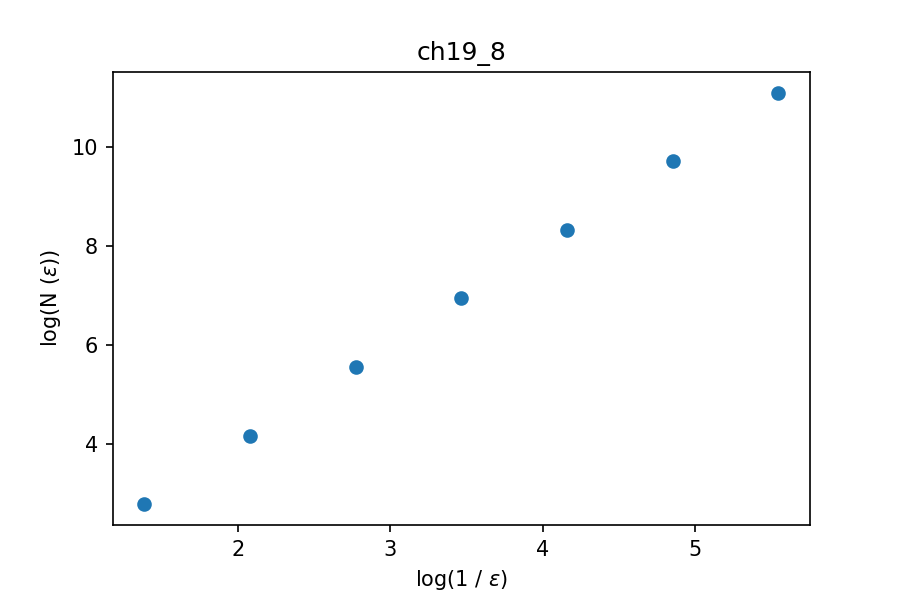
\includegraphics[scale=.35]{Ilustraciones/Cap_SFI_duplicates/chr_19_4.png}}
\end{minipage}

\caption{Gráficas del juego del caos aplicado a sub-cadenas del cromosoma 19. }
\label{fig:dim_ch19}
\end{figure}


%%%%%%%%%%%%%%%%%%%%%%%%%%%%%%%%%%
%%%%%%%%%%%%%%%%%%%%%%%%%%%%%%%%%%
%%%%%%%%%%%%  Random  %%%%%%%%%%%%
%%%%%%%%%%%%%%%%%%%%%%%%%%%%%%%%%%
%%%%%%%%%%%%%%%%%%%%%%%%%%%%%%%%%%

\begin{figure}[h!]

\centering
\begin{minipage}{.3\linewidth}
\centering
\subfloat[]{\label{main:a}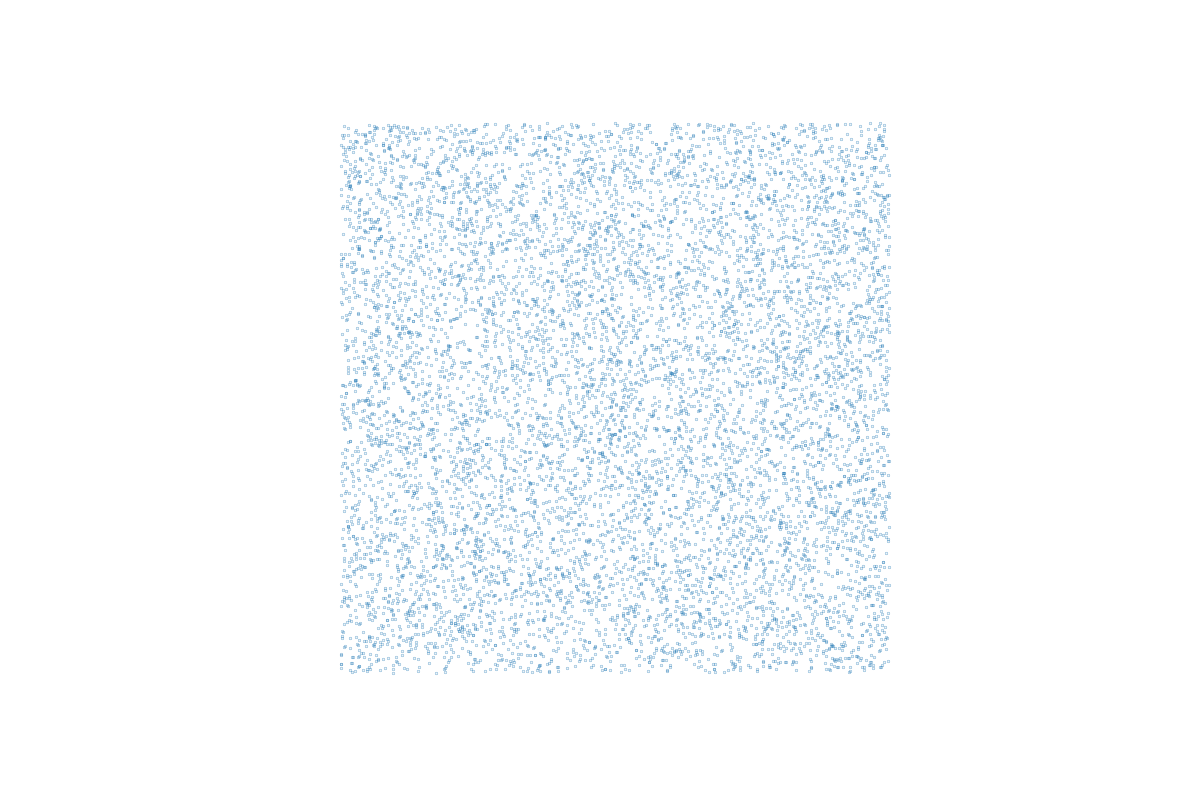
\includegraphics[scale=.45]{Ilustraciones/Cap_SFI/random_0.png}}
\end{minipage}%
\begin{minipage}{.3\linewidth}
\centering
\subfloat[]{\label{main:a}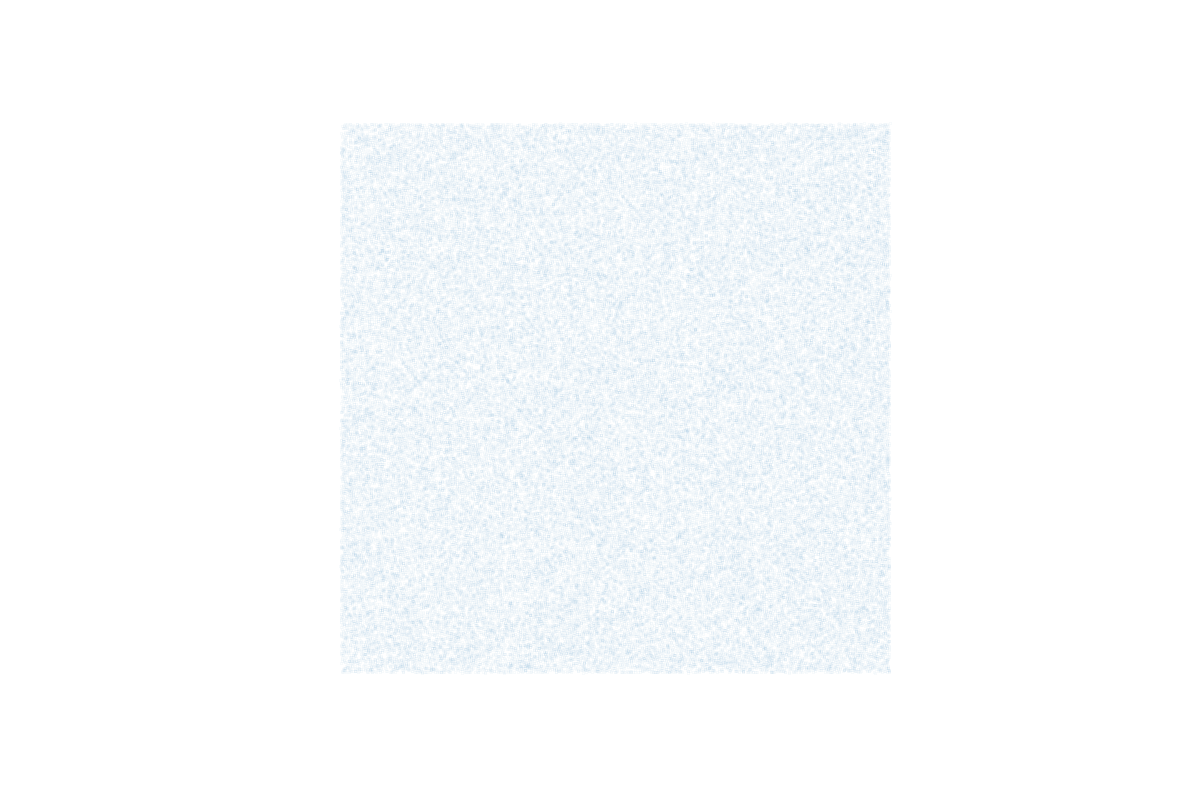
\includegraphics[scale=.45]{Ilustraciones/Cap_SFI/random_1.png}}
\end{minipage}%

\centering
\begin{minipage}{0.3\linewidth}
\centering
\subfloat[]{\label{main:a}
\includegraphics[scale=.45]{Ilustraciones/Cap_SFI/random_2.png}}
\end{minipage}%
\begin{minipage}{0.3\linewidth}
\centering
\subfloat[]{\label{main:a}
\includegraphics[scale=.45]{Ilustraciones/Cap_SFI/random_3.png}}
\end{minipage}

\caption{Gráficas del juego del caos en cadenas generadas aleatoriamente}
\label{fig:CG_random}
\end{figure}


\begin{figure}[h!]

\centering
\begin{minipage}{.3\linewidth}
\centering
\subfloat[]{\label{main:a}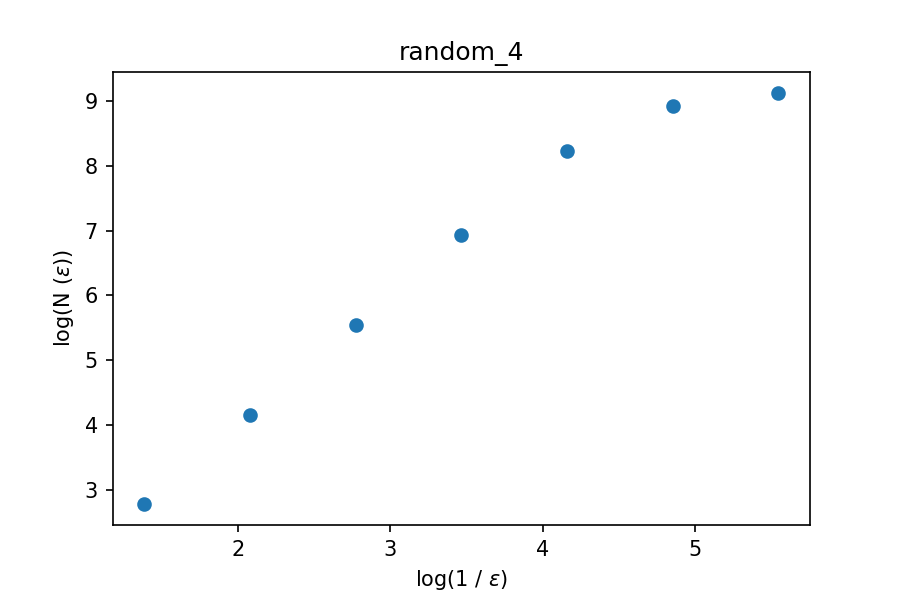
\includegraphics[scale=.35]{Ilustraciones/Cap_SFI_duplicates/0.png}}
\end{minipage}%
\begin{minipage}{.3\linewidth}
\centering
\subfloat[]{\label{main:a}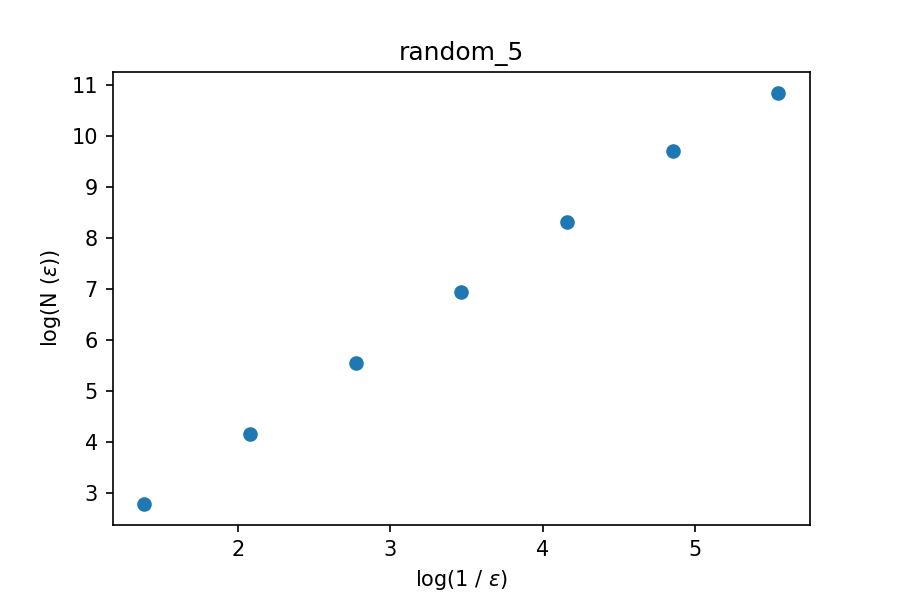
\includegraphics[scale=.35]{Ilustraciones/Cap_SFI_duplicates/1.png}}
\end{minipage}%

\centering
\begin{minipage}{0.3\linewidth}
\centering
\subfloat[]{\label{main:a}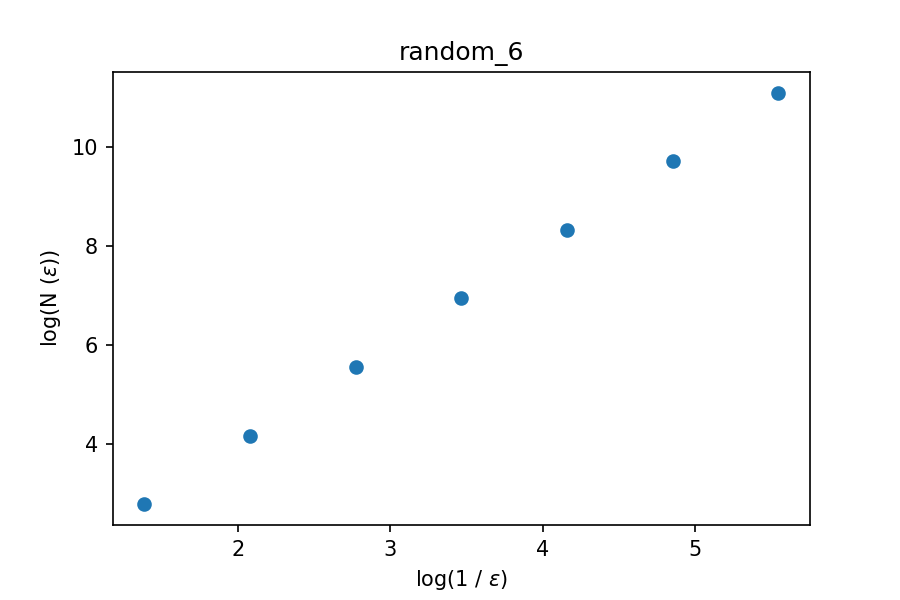
\includegraphics[scale=.35]{Ilustraciones/Cap_SFI_duplicates/2.png}}
\end{minipage}%
\begin{minipage}{0.3\linewidth}
\centering
\subfloat[]{\label{main:a}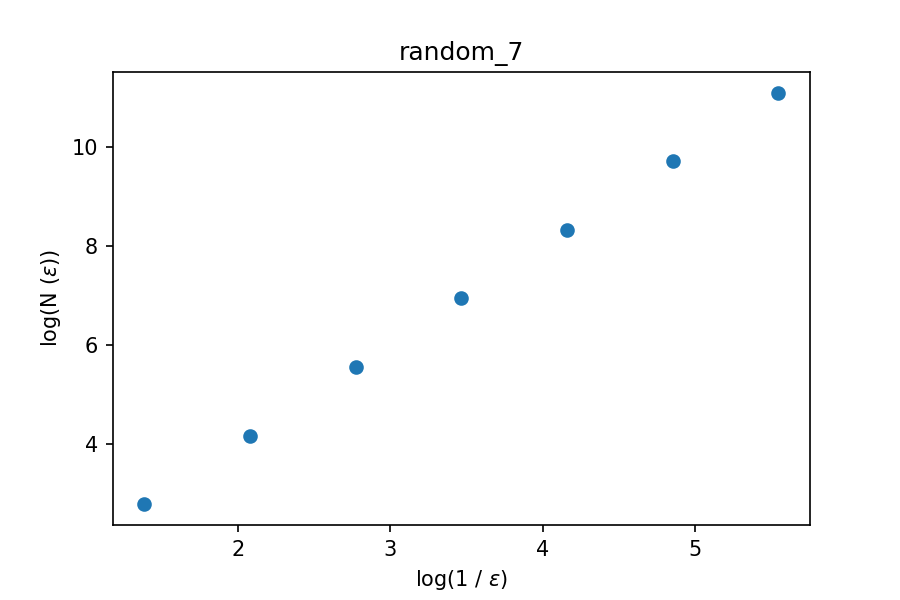
\includegraphics[scale=.35]{Ilustraciones/Cap_SFI_duplicates/3.png}}
\end{minipage}

\caption{Gráficas de la recta que se forma por la relación de la ecuación \ref{eq:dimfractal} en el conjunto de cadenas de caracteres aleatorios.}
\label{fig:dim_random}
\end{figure}
\\

En la tabla \ref{tab:dim} se incluyen las dimensiones aproximadas de los conjuntos anteriormente descritos para diferentes longitudes. $N$ se relaciona con la longitud de cada cadena según la ecuación: $len = 10^{N}$.
\\


%%%%%%%%%%%%%%%%%%%%%%%%%%%%%%%%%%
%%%%%%%%%%%%%%%%%%%%%%%%%%%%%%%%%%
%%%%%%%%%  Dimensiones  %%%%%%%%%%
%%%%%%%%%%%%%%%%%%%%%%%%%%%%%%%%%%
%%%%%%%%%%%%%%%%%%%%%%%%%%%%%%%%%%

\begin{center}
\begin{table}[]
    \caption{Dimensión de los conjuntos anteriormente descritos. \textit{str} representa el origen de los datos y \textit{N} se relaciona con la longitud de la cadena mediante la expresión: $len = 10^{N}$}.}
    \centering
    \begin{tabular}{lrr}
        \toprule
        \diagbox{N}{str} &  chr\_19 &  aleatoria \\
        \midrule
        \centering 4 &    1.56 &    1.61 \\
        5 &    1.90 &    1.96 \\
        6 &    1.99 &    2.00 \\
        7 &    2.00 &    2.00 \\
        8 &    2.00 &    - \\
        \bottomrule
        \end{tabular}
    \label{tab:dim}
\end{table}    
\end{center}


Se podría concluír que las dimensiones por conteo de cajas de ambos sistemas convergen a 2.0, el caso del juego del caos aplicado al DNA nunca llegó al valor de 2.0 sino que lo hizo después de que se redondeara a dos cifras después del punto decimal.
\\

También es menester considerar que, a juzgar por las figuras de los atractores del sistema mostrados en la figura \ref{fig:CG_chr19}, es posible que para subcadenas del cromosoma de gran longitud el sistema se esté saturando y la dimensión no sea la correcta.
\\

Para conocer acertadamente la dimensión de Minkowski-Bouligand, se calculó la dimensión para 500 subcadenas cuyas longitudes particionaran el intervalo $\[ 10^{5} , 10^{7} \]$ en 250 segmentos de igual tamaño. La gráfica de la longitud de la cadena vs la dimensión se muestra en la figura \textbf{incluir}.
\\

Notamos con esta figura que la, efectivamente, la dimensión se estabiliza rápidamente y se acerca asintóticamente a 2.0. Para determinar la dimensión real del sistema se propone:

\begin{itemize}
    \item Reducir la muestra a únicamente 50 puntos a partir de $10^{5}$.
    \item Seleccionar únicamente los primeros 10 y los últimos 10 puntos de la gráfica.
    \item Hacer una regresión lineal para cada uno de los dos segmentos anteriormente mencionados.
    \item Resolver el sistema de ecuaciones con los valores de las pendientes e interceptos del paso anterior.
    \item Determinar el punto sobre la curva de dimensiones que más se aproxime a la intersección entre las rectas del paso anterior.
\end{itemize}

Lo que se busca con esto es aproximar el punto de inflexión de la curva de dimensiones. Consideraremos este valor como la mejor aproximación de la dimensión de Minkowski-Bouligand para el juego del caos aplicado al cromosoma 19.


\subsubsection{Discusión}

De acuerdo con los resultados de la tabla \ref{tab:dim}, las dimensiones de Minkowski-Bouligand para juego del caos aplicado al cromosoma 19 y a cadenas aleatorias de caracteres parecieran converger ambos a 2.0.
\\

Si bien el punto al que convergen es el mismo, sí puede decirse que lo hacen a través de trayectorias diferentes. 
En las gráficas de las figuras \ref{fig:CG_chr19} y \ref{fig:CG_random} se muestran las gráficas con el mismo número de puntos y con las mismas dimensiones. Es evidente que juego del caos produce geometrías muy diferentes dependiendo del origen de las cadenas en que se aplicó el algoritmo; en \ref{fig:CG_chr19}, el llenado del cuadrado ocurre eventualmente aunque haya estados que el sistema no suela visitar (regiones con manchas blancas que se repiten con aparente regularidad en el cuadrado).
\\

Esto se corrobora con las dimensiones de la tabla \ref{tab:dim} donde la convergencia al 2.0 ocurra un orden de magnitud antes para el caso de la cadena aleatoria.
\\

El proyecto computacional completo con los métodos desarrollados para el cálculo de la dimensión así como varios ejemplos puede encontrarse \href{https://github.com/RobertoBastida/ChaosGame_DNA}{\emph{aquí}}. 




\begin{thebibliography}{9}



\bibitem{Análsis visual} Boeing, G. \textit{Visual Analysis of Nonlinear Dynamical Systems: Chaos, Fractals, Self-Similarity and the Limits of Prediction}. Systems 2016, 4, 37. 

\bibitem{Chaos on iterated function} 
M. Barnsley, A. Vince, \textit{The chaos game on a general iterated function system. Ergodic Theory and Dynamical Systems}, 31(4), 1073-1079. doi:10.1017/S0143385710000428, (2011)


\bibitem{Fractals Everywhere} M. Barnsley,  \textit{Fractals Everywhere} 2nd ed. Academic Press, Atlanta, Georgia, (1993).

\bibitem{fractals, chaos and power laws} M. Schroeder \textit{Fractals, chaos and power laws - Minutes from an Infinite Paradise} Freeman (1996).

\bibitem{Differential Equations} M. Hirsch, S. Smale, R. Devaney \textit{Differential Equations, Dynamical Systems and An Introduction to Chaos} 2nd ed. Elsevier Academic Press, 2004.


\bibitem{} M. Newville, et al. \textit{LMFIT: Non-Linear Least-Square Minimization and Curve-Fitting for Python}. Zenodo. 10.5281/zenodo.11813, 2014.

\end{thebibliography}

%\bibliographystyle{humannat}
%\bibliography{references}

\backmatter%@sglvgdor


\end{document}